%\documentclass[]{article}
\documentclass[11pt]{article}
\usepackage[usenames,dvipsnames]{xcolor}

\usepackage[T1]{fontenc}
%\usepackage{lmodern}
\usepackage{tgtermes}
\usepackage{amssymb,amsmath}
%\usepackage[margin=1in]{geometry}
\usepackage[letterpaper,bottom=1in,top=1in,right=1in,left=1in,includemp=FALSE]{geometry}
\usepackage{pdfpages}
\usepackage[small,labelfont=bf]{caption}
\usepackage{subcaption}
\usepackage{multirow}
\usepackage{longtable}
\usepackage{pdflscape}
\usepackage{array}
\usepackage{amssymb}
\usepackage{graphicx}

\newcolumntype{P}[1]{>{\raggedright\arraybackslash}p{#1}}
\usepackage{tikz}
\usetikzlibrary{mindmap, positioning}


\usepackage{ifxetex,ifluatex}
\usepackage{fixltx2e} % provides \textsubscript
% use microtype if available
\IfFileExists{microtype.sty}{\usepackage{microtype}}{}
\ifnum 0\ifxetex 1\fi\ifluatex 1\fi=0 % if pdftex
\usepackage[utf8]{inputenc}
\else % if luatex or xelatex
\usepackage{fontspec}
\ifxetex
\usepackage{xltxtra,xunicode}
\fi
\defaultfontfeatures{Mapping=tex-text,Scale=MatchLowercase}
\newcommand{\euro}{€}
\fi
%

\usepackage{fancyvrb}

\usepackage{ctable,longtable}

\usepackage{float} % provides the H option for float placement
\usepackage{dcolumn} % allows for different column alignments
\newcolumntype{.}{D{.}{.}{1.2}}

\usepackage{booktabs} % nicer horizontal rules in tables

%Assume we want graphics always
\usepackage{graphicx}
% We will generate all images so they have a width \maxwidth. This means
% that they will get their normal width if they fit onto the page, but
% are scaled down if they would overflow the margins.
%% \makeatletter
%% \def\maxwidth{\ifdim\Gin@nat@width>\linewidth\linewidth
%%   \else\Gin@nat@width\fi}
%% \makeatother
%% \let\Oldincludegraphics\includegraphics
%% \renewcommand{\includegraphics}[1]{\Oldincludegraphics[width=\maxwidth]{#1}}
\graphicspath{{.}}


%% \ifxetex
%% \usepackage[pagebackref=true, setpagesize=false, % page size defined by xetex
%% unicode=false, % unicode breaks when used with xetex
%% xetex]{hyperref}
%% \else
\usepackage[pagebackref=true, unicode=true, bookmarks=true, pdftex]{hyperref}
% \fi


\hypersetup{breaklinks=true,
  bookmarks=true,
  pdfauthor={Christopher Grady},
  pdftitle={Promoting Peace Amid Group Conflict: An Intergroup Contact Field Experiment in Nigeria},
  pdfkeywords = {group conflict, intergroup contact, Nigeria, field experiment},
  colorlinks=true,
  linkcolor=BrickRed,
  citecolor=blue, %MidnightBlue,
  urlcolor=BrickRed,
  % urlcolor=blue,
  % linkcolor=magenta,
  pdfborder={0 0 0}}

%\setlength{\parindent}{0pt}
%\setlength{\parskip}{6pt plus 2pt minus 1pt}
%\usepackage{parskip}
\setlength{\emergencystretch}{3em}  % prevent overfull lines
\providecommand{\tightlist}{%
  \setlength{\itemsep}{0pt}\setlength{\parskip}{0pt}}

%% Insist on this.
\setcounter{secnumdepth}{2}

\VerbatimFootnotes % allows verbatim text in footnotes

\title{Promoting Peace Amid Group Conflict: An Intergroup Contact Field
Experiment in Nigeria}

\author{\parbox{.7\linewidth}{\centering
Christopher Grady
}
}

\date{June 21, 2020}

\usepackage{versions}
\makeatletter
\renewcommand*\versionmessage[2]{\typeout{*** `#1' #2. ***}}
\renewcommand*\beginmarkversion{\sffamily}
  \renewcommand*\endmarkversion{}
\makeatother

\excludeversion{comment}

%\usepackage[margins=1in]{geometry}

\usepackage[compact,bottomtitles]{titlesec}
\setcounter{secnumdepth}{3}
%\titleformat{ ⟨command⟩}[⟨shape⟩]{⟨format⟩}{⟨label⟩}{⟨sep⟩}{⟨before⟩}[⟨after⟩]
\titleformat{\section}[hang]{\Large\bfseries}{\thesection}{.5em}{\hspace{0in}}[\vspace{-.2\baselineskip}]
\titleformat{\subsection}[hang]{\large\bfseries}{\thesubsection}{.5em}{\hspace{0in}}[\vspace{-.2\baselineskip}]
\titleformat{\subsubsection}[hang]{\bfseries}{\thesubsubsection}{.5em}{\hspace{0in}}[\vspace{-.2\baselineskip}]
%\titleformat{\subsubsection}[runin]{\bfseries}{\thesubsubsection}{1ex}{}[\vspace{-.2\baselineskip}]
\titleformat{\paragraph}[runin]{\bfseries\itshape}{\theparagraph}{1ex}{}{\vspace{-.2\baselineskip}}
%\titleformat{\paragraph}[runin]{\itshape}{\theparagraph}{1ex}{}{\vspace{-.2\baselineskip}}

%%\titleformat{\subsection}[hang]{\bfseries}{\thesubsection}{.5em}{\hspace{0in}}[\vspace{-.2\baselineskip}]
%%%\titleformat*{\subsection}{\bfseries\scshape}
%%%\titleformat{\subsubsection}[leftmargin]{\footnotesize\filleft}{\thesubsubsection}{.5em}{}{}
%%\titleformat{\subsubsection}[hang]{\small\bfseries}{\thesubsubsection}{.5em}{\hspace{0in}}[\vspace{-.2\baselineskip}]
%%\titleformat{\paragraph}[runin]{\itshape}{\theparagraph}{1ex}{}{\vspace{-.5\baselineskip}}

%\titlespacing*{ ⟨command⟩}{⟨left⟩}{⟨beforesep⟩}{⟨aftersep⟩}[⟨right⟩]
\titlespacing{\section}{0pc}{1.5ex plus .1ex minus .2ex}{.5ex plus .1ex minus .1ex}
\titlespacing{\subsection}{0pc}{1.5ex plus .1ex minus .2ex}{.5ex plus .1ex minus .1ex}
\titlespacing{\subsubsection}{0pc}{1.5ex plus .1ex minus .2ex}{.5ex plus .1ex minus .1ex}



%% These next lines tell latex that it is ok to have a single graphic
%% taking up most of a page, and they also decrease the space around
%% figures and tables.
\renewcommand\floatpagefraction{.9}
\renewcommand\topfraction{.9}
\renewcommand\bottomfraction{.9}
\renewcommand\textfraction{.1}
\setcounter{totalnumber}{50}
\setcounter{topnumber}{50}
\setcounter{bottomnumber}{50}
\setlength{\intextsep}{2ex}
\setlength{\floatsep}{2ex}
\setlength{\textfloatsep}{2ex}

\usepackage{setspace}
\doublespacing
\setlength{\parindent}{4em}

\begin{document}
\VerbatimFootnotes

%\begin{titlepage}
%  \maketitle
%\vspace{2in}
%
%\begin{center}
%  \begin{large}
%    PROPOSAL WHITE PAPER
%
%BAA 14-013
%
%Can a Hausa Language Television Station Change Norms about Violence in Northern Nigeria? A Randomized Study of Media Effects on Violent Extremism
%
%Jake Bowers
%
%University of Illinois @ Urbana-Champaign (jwbowers@illinois.edu)
%
%\url{http://jakebowers.org}
%
%Phone: +12179792179
%
%Topic Number: 1
%
%Topic Title: Identity, Influence and Mobilization
%
%\end{large}
%\end{center}
%\end{titlepage}


\maketitle


\newcommand\blfootnote[1]{%
  \begingroup
  \renewcommand\thefootnote{}\footnote{#1}%
  \addtocounter{footnote}{-1}%
  \endgroup
}
\singlespacing\blfootnote{Thanks to Jake Bowers, Jim Kuklinski, Justin Rhodes, Cara Wong, Caglayan
Baser, Ekrem Baser, Nuole Chen, Alice Iannantuoni, Betsy Rajala, Charla
Waeiss, and Donald Beaudette for useful conversations and feedback on
earlier drafts of this paper. Thanks to Danjuma Dawop, Lisa Inks,
Rebecca Wolfe, and the Mercy Corps Nigeria team for their work
implementing the peacebuilding project. Thanks to Tahiru Ahmadu, Ibrahim
Hassan, and the enumeration teams for their excellent work interviewing
farmers and pastoralists. Thanks to Hadiza Nuhu and Israel Okpe for
their work as the main contact people and mobilizers in farming and
pastoral communities.}

\begin{abstract}

Cooperative intergroup contact, originally designed as a tool for prejudice reduction, offers a promising means to resolve group conflict.  Evidence for contact-based interventions is sparse, however, and violent conflict may nullify the effects of contact.  We test the ability of a contact-based intervention to promote peace between conflicting groups with a field experiment in Nigeria, where farmer and pastoralist communities are embroiled in a deadly conflict over land use.  We evaluate the program with surveys, direct observation of behavior in markets, and a behavioral game.  We find that participation in the program increases intergroup trust, feelings of physical security, and voluntary intergroup contact measured both will self-reports and observed behavior in markets.  Many of the program's effects also diffuse to group members who did not directly participate in the program but who lived alongside participants. The program had no effect on a placebo outcome, attitudes towards violence, that one would expect to improve if the survey results were affected by social desirability bias.  These results suggest that reducing barriers to peace between conflicting groups is possible, and that structured intergroup contact is a promising method to do so.

\end{abstract}

\newpage

\hypertarget{introduction}{%
\section{Introduction}\label{introduction}}

How can groups in conflict improve intergroup relations? Violent group
conflict has caused 2 million deaths since the year 2000 (Sundberg and
Melander 2013), forcibly displaced over 70 million people from their
homes in 2018 (UNHCR 2019), threatens food supplies in numerous
countries (Verwimp and others 2012), and extracts a psychological toll
on participants and victims (Schomerus and Rigterink 2018). Intergroup
animosity perpetuates conflict long after the original grievance is
immaterial or forgotten (Deutsch 1973; McDonnel 2017; Tajfel and Turner
1979), so improving intergroup relations is vital to stem the human,
economic, social, and psychological costs of violent group conflict.

Scholars and practitioners consider \emph{cooperative} intergroup
contact -- contact in which members of two groups work together to
achieve common goals -- to be one of the most effective tools for
improving intergroup relations.\footnote{We will use the term
  \emph{cooperative contact} to refer to contact that meets Allport's
  conditions. Those conditions are (1) intergroup cooperation (2) with
  equal status (3) to achieve shared goals (4) with support of local
  authorities. Note that \emph{equal status} does not mean that the
  groups must have the same status in society, but that the groups share
  equal status in the cooperative situation. Cooperative contact stands
  in contrast to other forms of incidental or unstructured contact that
  may not have positive effects on intergroup relations.} Evidence for
the hypothesis that contact improves intergroup relations, known as the
contact hypothesis (Allport 1954), goes as far back as the 1950s and
motivated integrated public housing (Deutsch and Collins 1951) and
workplace and school desegregation (Cook 1985; Cook, Wrightsman, and
Wrightsman 1971; Slavin and Cooper 1999) in the United States. More
recent studies demonstrated the prejudice-reducing effects of contact by
leveraging random assignment to college dorms (Marmaros and Sacerdote
2006), college roommates (Boisjoly et al. 2006; Burns, Corno, and La
Ferrara 2015; Van Laar et al. 2005), schools (Rao 2019.), U.S. Air Force
groups (Carrell, Hoekstra, and West 2015), mixed sports teams (Ditlmann
and Samii 2016; Mousa 2018), job training programs (Scacco and Warren
2018), and medical doctors (Weiss 2019). The contact hypothesis also
increasingly motivates policy interventions, especially peacebuilding
programs (Ditlmann, Samii, and Zeitzoff 2017; Lemmer and Wagner 2015).

Despite contact's many successes, scholars know little about the effects
of contact-based interventions for people actively participating in and
personally victimized by a violent conflict, or even for interventions
directed at improving adults' attitudes towards racial or ethnic groups
(Paluck, Green, and Green 2019). Cooperative intergroup contact has only
recently been tested in the field, and never programmatically with
communities who are currently perpetrating violence against each other.
If one of the goals of cooperative contact is to mitigate violent
conflict, then contact-based interventions must be tested between
participants and victims in violent conflict.

Ongoing violence poses the most difficult test for contact and could
interfere with mechanisms through which contact improves relations. The
mechanisms through which contact improves relations assume that negative
attitudes result from unfamiliarity, and that ``familiarity breed{[}s{]}
liking'' (Pettigrew and Tropp 2006, 766). We posit that familiarity
through cooperative contact allows groups to identify latent shared
interests by providing positive interactions towards achieving a common
goal. Those positive interactions counter existing negative beliefs and
create cognitive dissonance (Festinger 1962; Tavris and Aronson 2008).
Attitudes improve when that cognitive dissonance is resolved by
rejecting negative beliefs rather than justifying negative beliefs
(Gubler 2013). However, by reinforcing negative beliefs and obscuring
shared interests, violent conflict could dull, prevent, or even reverse
the predicted positive effects of contact.

Despite these reasons for caution, there are reasons to expect
cooperative contact to improve intergroup relations even in contexts of
ongoing violence. Even in contexts of group violence, it is often in
each group's shared interest to reach a peaceful compromise because
fighting is costly (Fearon 1995). Cooperative contact to achieve a
common goal provides groups with an example of cooperation towards a
shared interest, and that experience can make groups imagine future
interactions for shared benefit. Cooperative contact can also remove the
psychological barriers to identifying shared interests, such as
stereotypes and feelings of threat and anxiety. Lastly, cooperation that
benefits the group should generate group pressure to cooperate, thus
creating cooperative social norms.

To learn about whether cooperative contact can improve intergroup
relations amidst violent group conflict, we conducted a field experiment
with conflicting farmer and pastoralist communities in Nigeria. More
than an occupational difference, farmers who cultivate crops and
pastoralists who graze cattle define a major social cleavage in many
parts of the world. These groups conflict over land rights, which define
both of their livelihoods. Farmer-pastoralist conflict has escalated
throughout the Sahel in recent years, and nowhere more than in Nigeria.
The most recent conflict escalation has caused 7,000 deaths from
2014-2019, displaced hundreds of thousands of people from their homes,
and costs \$13 billion annually in lost economic productivity (Akinwotu
2018; Daniel 2018; Harwood 2019; McDougal et al. 2015). In our sample,
some members of each community had been killed by members of the other
community in the year before the project began. Ongoing violence,
occupational and ethnic differences, and fighting over resources
necessary for livelihoods all make this context a hard test for contact
theory.

We randomly assigned communities with ongoing farmer-pastoralist
violence to receive a contact-based intervention or serve as a control
group. The intervention formed mixed-group committees and provided them
with funds to build infrastructure that would benefit both communities;
committees then collaboratively chose and constructed infrastructure
projects.\footnote{The communities built boreholes, market stalls, and
  primary health care facilities, for example.} The program also
provided mediation training to each community's leaders and held forums
where the groups discussed the underlying drivers of conflict. To
measure the effects of the intervention, we conducted pre- and
post-intervention surveys, a post-intervention natural public goods
behavioral game,\footnote{In a public goods game (PGG), research
  subjects are given money and told they can keep the money or donate it
  to a public fund. Money donated to the public fund is multiplied by
  some amount and then shared with all subjects. Our PGG is
  \emph{natural} because it was conducted in a natural setting, rather
  than a lab. The funding for the PGG came from the National Science
  Foundation under Grant No.~1656871.} and twelve months of systematic
observations in markets and social events during the intervention.

We find that the program increased intergroup affect, intergroup contact
outside of the intervention, and perceptions of physical security. We
see signs of the positive effects in fieldwork as well as in data: in
one of the treatment sites, farmers defended pastoralists from a group
of anti-pastoralist vigilantes, rather than assist the vigilantes in
removing the pastoralists and claiming their land. Our results also show
that the intervention affected communities as a whole, not just
community members directly involved in the intergroup contact.
Individuals who directly engaged in intergroup contact changed the most
positively from baseline to endline, but we also observe positive
spillovers of trust to group members for whom we did not exogenously
increase intergroup contact.

This study expands our knowledge about group conflict in two main ways.
First, this study teaches us about the capacity of intergroup contact to
improve intergroup relations and reduce conflict. Peacebuilding
organizations implement numerous contact-based interventions in violent
contexts each year, but its efficacy to improve intergroup attitudes
amid real-world conflict is an open question (Ditlmann, Samii, and
Zeitzoff 2017; Paluck, Green, and Green 2019). To our knowledge this is
the first field experimental test of a contact-based peacebuilding
intervention implemented during an active conflict. The results suggest
that contact-based peacebuilding programs can effectively improve
relationships between conflicting groups and is especially relevant to
conflict resolution in the cases of intergroup and intercommunal
conflicts.

Second, we contribute to the literature about informal structures, such
as social norms, in solving commitment problems. Many scholars have
identified group conflict as a commitment problem that is most likely to
be solved by an outside actor enforcing commitments (Fearon 1994). While
strong outside actors can resolve conflict by solving commitment
problems, this study suggests that they are not a necessary condition
for resolving conflict. Many communities in our treatment group
significantly improved their relations without a strong actor to enforce
commitments. Our results suggest that cooperative intergroup contact
helped groups strengthen their own conflict resolution structures.

\hypertarget{improving-intergroup-relations-through-cooperative-intergroup-contact}{%
\section{Improving Intergroup Relations Through Cooperative Intergroup
Contact}\label{improving-intergroup-relations-through-cooperative-intergroup-contact}}

Cooperative intergroup contact has long been posited as a means to
improve intergroup relations. Popularized by Gordon Allport (1954), the
contact hypothesis assumes that negative stereotypes cause intergroup
animosity. Stereotypes, natural mental shortcuts that help an individual
understand his/her experiences, are especially likely to go awry and
create animosity when an individual has little or no experience with
members of another group. Without intergroup experience, stereotypes
will misrepresent groups, create imagined differences between ingroup
and outgroup members, and obscure shared interests. To remove these
negative stereotypes new experiences must override them, allowing an
individual to re-conceptualize the outgroup.

Allport and subsequent authors specified four conditions under which
contact will remove stereotypes and improve intergroup relations. First,
the contact must involve ongoing personal interaction between members of
both groups. Second, both groups must have equal status in the
interaction. Third, the interaction must involve cooperation towards a
common goal. And fourth, the intergroup interaction must have the
support of, or at least not be punished by, institutions and
authorities. These conditions ensure positive interactions between group
members.

Allport argued that contact works by enhancing knowledge and overriding
negative stereotypes about the outgroup, and subsequent scholarship has
identified three additional mechanisms through which contact improves
attitudes. First, contact reduces the feelings of threat and anxiety
that arise from fear of the unknown (Page-Gould, Mendoza-Denton, and
Tropp 2008; Stephan and Stephan 1985). Second, contact enables
perspective-taking so that ingroup members empathize with the outgroup
(Batson et al. 1997; Broockman and Kalla 2016). And third, contact makes
salient a shared identity based on the groups' similarities and
interests (Gaertner and Dovidio 2014; Gaertner et al. 1993). Through
these mechanisms group members can experience positive cross-group
interactions, which triggers cognitive dissonance against the
preexisting negative attitudes. Attitudes improve when that dissonance
is resolved by rejecting, rather than justifying, negative attitudes
towards the outgroup (Gubler 2013).

These mechanisms support the reduction of group-based prejudice for
individuals involved in the intergroup interaction, but the positive
effects of contact must diffuse to individuals not involved in the
interaction for intergroup contact to meaningfully improve intergroup
relations. This diffusion to other group members occurs through changing
social norms about cross-group interaction (Christ et al. 2014; Paluck
2009) and through the knowledge that other ingroup members had positive
contact with outgroup members (Wright et al. 1997). Norms and awareness
of cross-group cooperation shows that cross-group interaction is safe
and socially encouraged. It also creates the expectation of future
interaction with outgroup members, which motivates individuals to see
the outgroup more positively (Klein and Kunda 1992; Van Dessel, Hughes,
and De Houwer 2019). Through social diffusion cooperative contact
improves attitudes even for ingroup members with no cross-group contact.

Taken together, the existing literature suggests that cooperative
contact improves intergroup relations through four steps. First,
cooperative contact provides positive interactions that remove the
psychological barriers -- negative stereotypes, feelings of outgroup
threat, and a lack of empathy -- that bias perceptions of the other
side. Second, without these perceptual biases groups can identify shared
interests, and cooperative contact facilitates the identification of
shared interests by having the groups cooperate towards a common goal.
Third, positive interactions and the identification of shared interests
challenge pre-existing negative beliefs and trigger cognitive
dissonance. Attitudes improve when that dissonance is resolved by
rejecting preexisting negative attitudes in lieu of new positive
experiences. Fourth, positive attitudes diffuse to other group members
through awareness of cross-group cooperation and changing social norms.

\hypertarget{cooperative-intergroup-contact-in-the-context-of-violent-group-conflict}{%
\subsection{Cooperative intergroup contact in the context of violent
group
conflict}\label{cooperative-intergroup-contact-in-the-context-of-violent-group-conflict}}

Violent group conflict poses a hard test for cooperative intergroup
contact to improve attitudes. First, in the context of ongoing violent
conflict, even cooperative contact towards a joint goal may not provide
group members with a subjectively positive cross-group interaction. Due
to psychological biases, individuals perceive cross-group interactions
negatively so that those interactions conform to pre-existing beliefs;
individuals also more readily store and recall negative interactions
that confirm pre-existing attitudes than positive interactions that are
dissonant with pre-existing attitudes (Nickerson 1998; Ward et al.
1997). If individuals perceive cooperative contact negatively, contact
could make attitudes worse, not better (Barlow et al. 2012; Paolini,
Harwood, and Rubin 2010; Stark, Flache, and Veenstra 2013).

Even if contact succeeds in providing positive experiences with outgroup
members, the resulting cognitive dissonance may not be resolved by
embracing positive attitudes. Participation in and victimization by
violence motivates group members to justify their existing attitudes
(Kunda 1990). Existing attitudes are harder to reject once an individual
has acted on them (Festinger 1962; Tavris and Aronson 2008). Once an
attitude is acted upon, rejection of the attitude threatens an
individual's self-identity because the the individual must come to terms
with his or her own immoral behavior. Likewise, individuals are less
likely to reject existing attitudes when they have personal experiences
that reinforce those attitudes. In the case of prejudice, prejudiced
attitudes are least likely to be rejected when an individual has harmed
or been harmed by the outgroup. Instead of rejecting negative attitudes,
violent experiences can lead individuals to resolve cognitive dissonance
by justifying previous attitudes (Gubler 2013) or, at best, by
differentiating ``good'' outgroup members from typical outgroup members
(Doosje, Spears, and Koomen 1995).

Beyond past violent, ongoing group violence provides negative
experiences with outgroup members that counter the positive experiences
provided by cooperative contact. These negative experiences bolster the
psychological barriers to groups' identifying their shared interests.
Rather than dispelling stereotypes and alleviating feelings of threat,
negative experiences reinforce negative stereotypes and justify feelings
of threat. Taking the perspective of the other side will not improve
cross-group relations if taking their perspective reveals incentives for
belligerence (Kertzer, Brutger, and Quek 2018). And far from revealing
common identities and interests, group violence perpetuates opposing
group identities and interests (Fearon and Laitin 2000). To overcome
preexisting negative beliefs, individuals need strong and consistent
information that counters those existing beliefs -- a signal that the
object of their belief has changed (Nickerson 1998). For that reason,
some scholars believe group reconciliation cannot begin until conflict
is resolved (Bar-Tal 2000).

Social norms are a potent means to change attitudes and behavior, but in
contexts of group violence social norms prevent rather than facilitate
attitude change (Bar-Tal 2007; Bar-Tal and Avrahamzon 2017). These
pre-existing norms self-perpetuate by discouraging ingroup members with
positive attitudes from displaying those attitudes, either through
talking about or engaging in cross-group interaction publicly. Group
members who do not conform to these norms risk being branded as traitors
(Bornstein 2003). With no opportunities to hear about or observe
positive cross-group interaction, the effects of contact cannot extend
to ingroup members without contact.

But these barriers do not mean that contact cannot improve intergroup
relations for groups in violent conflict. Conflicting groups share an
interest in obtaining peace because fighting is costly (Fearon 1995),
and cooperative contact can make that shared interest salient. Though
existing norms likely support negative attitudes, successful cross-group
cooperation can generate cooperative social norms because cooperation
and peace are in the interest of both groups. Cooperative contact also
shows that the outgroup is composed of differentiated individuals (Rimé
et al. 2011), opening the possibility that past negative experiences
with a few outgroup members do not characterize the entire outgroup.

\hypertarget{farmer-pastoralist-conflict-in-nigerias-middle-belt}{%
\section{Farmer-pastoralist conflict in Nigeria's Middle
Belt}\label{farmer-pastoralist-conflict-in-nigerias-middle-belt}}

Nigeria's Middle Belt is plagued by violent conflict over land use.
Farmers, who claim land for agricultural production, and pastoralists,
who claim land for animal grazing, increasingly clash over claims to the
same land. Both groups depend on land for their livelihoods, but their
divide is also cultural, ethnolinguistic, and, in some locations,
religious. The pastoralists are almost homogeneously of the Fulani
ethnic group, speak Fulfulde as their primary language, and practice
Islam. They maintain a semi-nomadic way of life, belonging to a home
community but traversing vast distances to secure access to pastureland
and water as seasons change. The farmers live in sedentary villages and
exploit land for agriculture. The ethnic group, language, and religion
change by village. In our study, farmers came from more than a dozen
ethnic groups, often residing in the same village.

Historically, these communities cooperated through trade and sharing
land that was abundant relative to populations. Pastoralists would graze
their animals on crop residue after harvests and follow migration paths
away from farmland during planting seasons. The groups were
complementary: pastoralists gained food for their animals and farmers
gained animal manure/urine to replenish soil; farmers bought milk and
meat from pastoralists and pastoralists bought grains and vegetables
from farmers. There were tensions, but these were typically overcome by
negotiation and violence seems to have been rare. The Middle Belt came
to be known as Nigeria's ``food basket'' due to the abundance of
foodstuffs coming out of the region, like beef, dairy, yam, and
cassava\footnote{\url{https://qz.com/africa/1315749/nigeria-herdsmen-farmer-attacks-are-damaging-agriculture-economy/}}.

In recent years, this relationship has been stressed by populations
booms and climate change. Nigeria's population at independence in 1960
was about 50 million; Nigeria's population in 2019 is estimated around
200 million. At the same time, the Sahara's size expanded over 10\%,
decreasing land available for farming and grazing (Okpara et al. 2015;
Thomas and Nigam 2018). As the number of farmers, pastoralists, and
mouths to feed increased, the amount of land available to produce food
declined. These factors also pushed pastoralists southward, towards
farming communities with whom the pastoralists had no pre-existing
relationship. Land scarcity and new migrants jeopardize traditional
cooperative agreements that have managed farmer-pastoralist interactions
for decades (Cotula et al. 2004; Kuusaana and Bukari 2015). Sharing land
is easier when people are scarce and land is plentiful; it is not so
easy when land is scarce and people are plentiful.

Government policies exacerbated the issues caused by demographic and
geographic changes. Land privatization encouraged farmers to plant crops
that occupy land continuously, like orchards, and effectively nullified
farmer-pastoralist land sharing agreements (Bassett 2009). Official
cattle reserves for moving herds are rarely enforced by the government,
leading farmers to plant crops in once-protected areas and further
limiting pastoralists' available grazing space. The ``indigene versus
settler'' policy limits economic and political rights to certain ethnic
groups in each state, often denying the ``settler'' pastoralists the
ability to own land and run for political office (Network 2014).

These stressors have sparked violent conflict between farmers and
pastoralists in recent years (Ilo, Ier, and Adamolekun 2019). The most
recent conflict escalation, beginning roughly in 2014, has caused 7,000
deaths (Harwood 2019) and displaced hundreds of thousands of people from
their homes (Akinwotu 2018; Daniel 2018). The scale of economic damage
is unknown, but farmer-pastoralist conflict \emph{before} this
escalation cost Nigeria \$13 billion annually in lost economic
productivity (McDougal et al. 2015). This violence has impeded food
production, leading to an impending food crisis (Hailemariam 2018; Ilo,
Ier, and Adamolekun 2019; Unah 2018). Compounding matters, state
governments' response to the conflict has been to enact anti-grazing
laws. These laws spark more violence because many pastoralists
reasonably viewed the law as biased against their way of life. In the
state of Benue, the government mobilized state-sanctioned vigilante
groups called ``livestock guard'' to enforce the law, but the livestock
guard have sometimes sought out pastoralists, rather than guard farmland
(Duru 2018).

Though we have discussed the conflict as between two large and cohesive
groups (``Farmers'' and ``Pastoralists''), the conflict occurs between
numerous small, independent farming and pastoral groups. The groups
typically reside a couple miles from each other -- like people from the
next town over. These independent groups are aware of the broader
context of farmer-pastoralist conflict, but their concerns are local and
mostly unrelated to what happens in distant villages. Different versions
of the same story initiate and sustain the local conflicts. First,
cattle graze on farmland.\footnote{In past decades, compensation for
  crop damage would have been standardized, but these traditional
  agreements have fallen apart in recent years (Cotula et al. 2004;
  Kuusaana and Bukari 2015). With no agreed upon compensation and no
  authority to punish illegal grazing or illegal cattle rustling, groups
  take justice into their own hands.} Next, a farmer retaliates by
stealing cattle from the pastoralists (because the farmer does not know
\emph{which} herd grazed on his land, the stolen cattle do not
necessarily come from the transgressing herd). This cycle continues and
eventually explodes when a member of one side physically attacks a
member of the other side. From there, a little war often breaks out. As
one reporter noted, ``The countryside is littered with the charred ruins
of homes, schools, police stations, mosques and churches.'' (McDonnel
2017).

Farmer-pastoralist conflict poses a tough test for intergroup contact to
improve group relations. The material, social, and psychological
incentives of these groups are opposed. They want the same land for
different purposes and their livelihoods depend on that land. The groups
are involved in a bloody, violent, and escalating conflict for land in
which thousands of farmers and thousands of pastoralists have been
killed by members of the other group. Within an individual's community,
several people will have been attacked or killed; several others will
have attacked or killed members of the other side. To justify killing,
groups create collective myths about the retaliatory/defensive nature of
their belligerent action and the iniquity and inhumanity of the other
side. Despite their physical proximity, the groups have little to bond
over; they are distinct culturally, ethnically, linguistically, and
often religiously. And finally, government favoritism of farmers over
pastoralists creates a power disparity between the groups.

Despite the forces pushing these groups into conflict, their interests
are not completely misaligned. Peace is in the interest of both groups
because fighting is costly, both materially and psychologically. The
conflict has destroyed billions of dollars in agricultural produce,
animal products, and physical infrastructure. Crops have been destroyed,
cattle stolen, homes burned, and neighbors murdered. Farmers fear
violence when working in their fields; pastoralists fear violence when
grazing their cattle. Peace can end the economic, social, and human
costs. Moreover, the groups formerly maintained mutually beneficial
trade agreements: farmers trade the crop residue left on their fields
for animal manure/urine to replenish soil; farmers traded grains and
vegetables in exchange the pastoralists' milk and meat. Peace rekindles
the possibility of these mutually-beneficial trade agreements.
Cooperative intergroup contact should improve group relations by
revealing these shared interests.

Farmer-pastoralist conflict is not confined to Nigeria's Middle Belt.
Farmer-pastoralist clashes are a persistent problem throughout the Sahel
and savanna areas of Africa, including Mali, the Ivory Coast (Bassett
1988, 2009), Niger (Thebaud and Batterbury 2001), and Ghana (Tonah
2002). Farmer-pastoralist clashes are destabilizing to these countries
politically, socially, and economically. Similar group dynamics exist in
Europe with Roma, an outgroup viewed as culturally, ethnically, and
linguistically distinct and apart from the rest of the polity. Similar
conflict dynamics exist between Jews and Arabs, who also conflict over
land that both groups claim. Scholars can learn about intergroup
conflict generally from farmer-pastoralist conflict in Nigeria's Middle
Belt.

\hypertarget{intervention-engaging-communities-for-peace-in-nigeria}{%
\subsection{Intervention: Engaging Communities for Peace in
Nigeria}\label{intervention-engaging-communities-for-peace-in-nigeria}}

To address farmer-pastoralist conflict, peacebuilding NGO Mercy Corps
implemented a four-year, USAID-funded program titled Engaging
Communities for Peace in Nigeria (ECPN) in Middle Belt sites embroiled
in violent conflict. The main objective of the program was to foster
positive contact between farmers and pastoralists, improve attitudes,
improve intergroup relations, and ameliorate conflict. Mercy Corps
implemented the project in two Middle Belt states, Benue and Nassarawa,
which have been focal points for farmer-pastoralist conflict.

The intervention formed mixed-group committees with equal numbers of
farmers and pastoralists and provided them with funds to build
infrastructure that would benefit both communities; committees then
collaboratively chose and constructed infrastructure projects. It
started with separate farmer and pastoralist community meetings to avoid
negative contact experiences. These intra-community meetings eventually
built up to joint decision-making meetings with the two groups together.
Each joint project committee included an even number of farmers and
pastoralists, as well as women and youth representatives, and totaled
between 12 and 15 members. Each committee received two grants, one for
quick-impact projects, of approximately \$2,000, and one for joint
projects, of approximately \$25,000.

The quick-impact projects were conceived as a trust-building initiative,
intended to let community members see that cooperation was possible.
Projects, managed by both farmers and pastoralists, included hand pumps;
construction or rehabilitation of market stalls, schools, and health
centers; and construction of fences along grazing routes to protect
farmlands and avoid accidental crop damage. The joint economic
development projects aimed to address an underlying issue related to the
conflict: sharing of resources that impact livelihoods. Pollution of
water, affecting both farming and livestock, was the primary issue
people raised. As a result, each site chose to build a new borehole
well, with members of both farmer and pastoralist communities helping to
construct the wells.

To ensure support of authorities, the program involved community leaders
from both sides in all aspects of the project. They were involved in the
quick-impact projects and joint economic development projects. We also
provided mediation training to each community's leaders and held forums
where the groups discussed the underlying drivers of conflict.

These projects were designed with the conditions of Contact Theory in
mind. Groups (1) cooperated with (2) equal status to achieve (3) shared
goals with (4) support of local authorities. These projects were meant
to help the groups solve, through intergroup cooperation, problems
relevant to both groups. This would reveal to groups that they shared
many of the same struggles and that cooperation could help them overcome
these struggles. Collectively, these project give groups the opportunity
so send costly signals about their willingness to cooperate (Kydd 2000,
@rohner2013war).

In the next section we describe the research design to determine the
effects of intergroup contact on intergroup attitudes and behaviors.

\hypertarget{research-design}{%
\section{Research Design}\label{research-design}}

We evaluate the effects of Engaging Communities for Peace in Nigeria
(ECPN) with a site-level field experiment. Each site contains two
communities, one of farmers and one of pastoralists. The communities
within a site engaged in deadly clashes within one year of our scoping
exercise.\footnote{To identify eligible sites, we undertook a scoping
  exercise to determine if the two communities in an implementation site
  had a demonstrated need for a peacebuilding program and were willing
  to participate in one. We defined ``demonstrated need'' as the
  communities engaging in violent clashes within one year of the scoping
  exercise. Willingness to participate in the program was obtained
  through conversations with community leaders, none of whom refused the
  program.} We identified fifteen sites eligible for the study and
surveyed \textasciitilde{}50 randomly selected respondents per
community. We then randomly selected the communities in ten of fifteen
sites to receive the ECPN program, blocking by state so that an equal
proportion of sites in Benue and Nassarawa received the program. After
18 months, we surveyed another \textasciitilde{}50 randomly selected
respondents and \textasciitilde{}10 respondents from the baseline survey
per community. In between the surveys, we monitored farmer-pastoralist
interactions in markets and at social events.\footnote{This experimental
  design was pre-registered with Evidence in Governance and Politics
  (EGAP) under ID 20150716AA. The preregistration can be found at
  \url{http://egap.org/registration/1242}.}

This designs gives us two datasets to analyze. First, we aggregate the
randomly-sampled individuals to compare communities before and after
ECPN. The main goal of this analysis is to learn about the effect of
implementing ECPN in a community. Communities were randomly assigned to
receive ECPN or function as a control group, which allows us to
determine the causal effect of ECPN at a community-level. This
comparison between communities that received or did not receive ECPN is
our main analysis.

Second, we supplement the community-level analysis by creating a dataset
of \textasciitilde{}10 respondents per community before and after ECPN.
The main goal of this analysis is to learn about the effect of
participating directly in ECPN committees, and thus directly
experiencing intergroup contact, relative to the effect of living in
communities where ECPN was implemented but not participating in
committees, and thus only experiencing indirect intergroup contact. From
our baseline random sample, we identified and resurveyed (1) ECPN
committee participants, (2) respondents who lived in intervention sites
but did not participate in ECPN committees, and (3) respondents from the
control group, who neither participated in ECPN committees nor lived in
communities where ECPN was implemented. We then compare the change of
participants and nonparticipants in intervention sites to the change in
control respondents. Our ability to make generalizable causal claims
about participation is limited, though, because individuals in
intervention sites were not randomized into participation or
nonparticipation with ECPN committees.\footnote{We initially randomly
  assigned baseline survey respondents to be part of ECPN committees,
  but random assignment proved difficult. Many people who were not
  selected wanted to be on the committees, and some people who were
  selected were not able to participate or could not be located when the
  committees were launched. As a result, people self-selected into
  committees.}

In total, we randomly sampled 1539 respondents at baseline in 2015. 1027
of those respondents were in intervention sites and 512 were in control
sites. At endline, we resurveyed 287 of those respondents. 74 of those
respondents directly participated in ECPN, 121 were in intervention
sites but did not participate, and 92 were in control sites. At endline,
we also randomly sampled 1523 respondents, 1028 in intervention sites
and 295 in control sites.

\hypertarget{estimation}{%
\subsection{Estimation}\label{estimation}}

Here we describe our estimation procedure for the community-level
analysis and the individual-level analysis. For both analyses we
estimate one-tailed tests because our hypotheses are that the change in
outcomes for treatment units will be \emph{greater than} control, not
that the change in outcomes for treatment units will be \emph{different}
than control. Both analyses also use randomization inference for
\(p\)-values and bootstrapping for standard errors. The specifics of
each procedure are described in Appendix A.

We use two estimators to estimate the treatment effect of ECPN. When
treatment groups are balanced on the baseline outcome, we use the
baseline outcome as a covariate to predict the endline outcome, as seen
in equation 1. When treatment groups are not balanced on the baseline
outcome, we use the change score of the outcome as Y, as seen in
equation 2.\footnote{We use two different equations because the
  effectiveness of each equation depends on the correlation between
  treatment assignment and baseline outcomes. The ``controlling-for''
  method of equation 1 is more precise but is biased when treatment
  assignment correlates with baseline outcomes. The ``differencing''
  method of equation 2 is unbiased but less precise. For a comparison
  between these methods, see
  \url{https://declaredesign.org/blog/2019-01-15-change-scores.html}.}

\medskip

\(Y_{i,j} = \beta_0 + \beta_1Z_{i,j} + X_{i,j} + \delta_j + \epsilon_{i,j}\)

\medskip

\noindent Where \(i\) is the community in state \(j\), \(Z\) is the
treatment indicator, \(X\) is the outcome at baseline, and \(Y\) is the
outcome at endline. \(\delta\) is a fixed effect for the state \(j\) in
which the community belongs.

\medskip

\(Y_{i,j} = \beta_0 + \beta_1Z_{i,j} + \delta_j + \epsilon_{i,j}\)

\medskip

\noindent Where \(i\) is the community in state \(j\), \(Z\) is the
treatment indicator, and \(Y\) is the change in outcome from baseline to
endline. \(\delta\) is a fixed effect for the state \(j\) in which the
community belongs.

We use randomization inference for \(p\)-values and bootstrapping for
standard errors because our units of analysis, communities and
individuals, are clustered in sites and we have only fifteen sites.
Analytic standard errors may underestimate the uncertainty of our causal
estimate. Bootstrapping yields a distribution of possible treatment
effects given the observed data, and the 95\% confidence interval is
between the coefficients at the 2.5th percentile and the 97.5th
percentile.

\hypertarget{outcomes}{%
\subsection{Outcomes}\label{outcomes}}

We measured three outcomes to estimate the effect of ECPN: (1)
intergroup attitudes, (2) intergroup contact, and (3) insecurity. If
ECPN improved intergroup relations, we would expect respondents to
report better attitudes towards the outgroup, more intergroup contact
and willingness to engage in intergroup contact, and reduced insecurity
due to violence. We also measured three mechanisms from the contact
literature through which contact could affect outcomes: (1)
empathy/perspective-taking, (2) perceived threat, and (3) ingroup
expansion. Lastly, we measured a placebo outcome that may be affected by
social desirability: attitudes about violence. We measured these
outcomes with survey self-reports, survey experiments, a natural-field
behavioral game, and monitoring of farmer-pastoralist interaction in
markets and social events.

For most survey self-reports, we combine together several survey
questions to create an index. We create both additive indices and
inverse-covariance weighted indices. Inverse-covariance weighting
constructs an index by down-weighting index questions that are
correlated with other index questions and up-weighting those that are
uncorrelated with other questions. This approach maximizes the amount of
unique information the index takes from each question and prevents
``double counting'' when two questions measure the same underlying
concept. We report results using inverse-covariance weighted indices,
but results hold with additive indices. Results with additive indices
are included in Appendix B.

\hypertarget{primary-outcomes}{%
\subsubsection{Primary outcomes}\label{primary-outcomes}}

\textbf{Intergroup affect}: Our first outcome is affect towards the
other side. A primary goal of our contact intervention, and of much
previous contact research, was for individual's attitudes to improve,
Changing attitudes towards the other side is one pathway towards
improving intergroup relations and changing behavior, though not the
only pathway (Paluck 2009; Scacco and Warren 2018).

We measure intergroup affect with survey self-reports and an endorsement
experiment. The survey questions include two measures of intergroup
trust and a five item social distance scale created for the
farmer-pastoralist context.

In an endorsement experiment, respondents are asked how much they
support a hypothetical policy. In the treatment condition, the policy is
`endorsed' by a group that the respondent has a positive or negative
opinion about. In the control condition, the policy is not endorsed by
any group. The average difference in support between the endorsed and
unendorsed policy represents the change in support for the policy
because of the group's endorsement. In our case, we asked respondents
how much they would support a water policy if it was endorsed by a
farmer organization (asked of pastoralists), if it was endorsed by a
pastoralist organization (asked of farmers), or if no endorsement was
mentioned (the control condition posed to both pastoralists and
farmers). Support was measured on a 5-point scale, where high values
indicated support and low values indicated opposition.

\textbf{Intergroup contact}: Our second outcome is intergroup contact
that occurs outside of the intervention. Natural, voluntary intergroup
contact provides behavioral evidence that farmer-pastoralist relations
are improving. We measure intergroup contact with survey self-reports,
monitoring of farmer-pastoralists interactions in markets and social
events, and a survey experiment.\footnote{Much of the self-reports and
  the observations are overdispersed count data. We recode all count
  data as rank.}

The self-reports and behavioral observations tell us the real,
descriptive change in intergroup contact. The survey self-reports ask if
and how often the respondent interacted with the other group in the past
month. The respondents are asked about interaction in markets, at public
social events, in the respondent's own home, at the home of a member of
the other group, and in any other way. The responses are then ranked,
scaled from 0-1, and combined into an index. The behavioral observations
provide a measure of contact independent of response biases.

In the markets, we measured interactions related to buying and selling
market goods, such as the number of farmer and pastoralist sellers
present and the number of farmer and pastoralist buyers. We then create
a farmers index and a pastoralist index to measure the presence of
farmers and pastoralists in the market. At social events, we measured
the number of members of the other group in attendance and the number
who ate or drank anything\footnote{Taking food or beverages at a social
  event is a sign of closeness and intimacy in these contexts. Casual
  attendees would not take food or beverages}, both in absolute numbers
and as a percentage of total attendees. We then create measures for the
number of farmers and pastoralists attending social events and the
number of farmers and pastoralists eating at social events.\footnote{Observations
  were made in two periods: July 2016 -- February 2017, immediately
  after the project commenced but before joint project committees
  convened, and September 2017 -- December 2017, after project
  committees convened but before the endline survey began. Events that
  occurred February 2017 or earlier are baseline measurements; events
  occurring September 2017 or later are endline measurements.}

A survey experiment, which we are calling the \emph{percent experiment},
tells us about respondents' willingness to engage in contact. It asks
respondents two questions about their willingness to interact with
members of the other side. We asked respondents if they would (1) join a
group and (2) live in a community with some percentage of the other
group. The percentage is randomized between 5\%, 25\%, 50\%, and 75\%;
the percentage is the same for those two questions but varies across
individuals. We take the mean response so that a respondent saying yes
to both is assigned a 1, a respondent saying yes to one is assigned a
0.5, and a respondent saying no to both is assigned a 0. These questions
allow us to determine if treatment communities become more willing to
interact with outgroup members and if treatment communities become less
sensitive to higher proportions of the outgroup.\footnote{This
  experiment was based on a question from the GSS asking respondents if
  they would favor or oppose living in a neighborhood that was half
  white/black.}

\textbf{Insecurity}: Our third outcome is feelings of insecurity due to
conflict. The end goal of ECPN is to reduce conflict between farmers and
pastoralist. The disaggregated and diffuse nature of the conflict makes
obtaining an accurate measure of violent conflict extremely
difficult.\footnote{Asking respondents to recount the number of violent
  events does not accurately measure the scale of the conflict because
  those answers are determined by the awareness and memory of the
  community members. Awareness of individual violent events is low
  because many of the violent events occur in fields and grazing routes
  far from the town center and residential areas. In addition, ECPN
  sought to increase awareness of violent events through its conflict
  forums. The type of event that all community members are aware of --
  large massacres, burning of homes, etc\ldots{} -- generally lead to
  the disintegration of both communities as community members flee the
  area fearing further violence or reprisals. These large-scale events
  are rare and none occurred in intervention or control communities
  during the study.} Instead, we measured the effect that violent
conflict has on individuals. We ask respondents if they avoid any areas
during the day or night due to insecurity and if insecurity restricted
them from engaging in various activities, such as grazing their animals,
working on their farms, fetching water for their families, and working
for wages. We combined these ten insecurity questions into an index,
with high values indicating low perceptions of insecurity and low values
indicating high perceptions of insecurity.

\textbf{Violence Placebo}: Several of our outcomes are survey
self-reports, and all self-reports could be affected by social
desirability bias. Our survey results are suspect if respondents in
treatment communities learned the ``correct'' answers better than
respondents in control communities. If social desirability accounts for
the effect in survey self-reports, we would also expect differences
between treatment and control for other normatively desirable attitudes.
To test social desirability effects, we conduct a placebo analysis using
attitudes about violence as a placebo. Attitudes about violence are a
good candidate for a placebo because intergroup contact should not
affect general attitudes about violence, but respondents may feel social
pressure to answer violence questions in a desirable way. We measure
attitudes about violence with a six question index asking respondents if
it is always, sometimes, rarely, or never justified to use violence in
certain situations, such as retaliating against violence or bringing
criminals to justice.

\hypertarget{mechanisms}{%
\subsubsection{Mechanisms}\label{mechanisms}}

The primary outcomes of intergroup affect, intergroup contact, and
insecurity tell us if ECPN worked but provide no evidence for how the
program worked. Previous work on contact specified three mechanisms
through which contact affects attitudes: empathy/perspective-taking,
threat/anxiety, and ingroup expansion (Al Ramiah and Hewstone 2013;
Dovidio et al. 2017; Pettigrew and Tropp 2008). We do not manipulate
these mechanisms directly, and so cannot make causal claims about the
mediating role of these variables for ECPN. But we can provide
exploratory evidence that these mechanisms played a role if (1) ECPN
affects these mechanisms and (2) these mechanisms affect intergroup
affect, intergroup contact, and insecurity.

\textbf{Threat}: We use three self-report survey questions to measure
threat felt by the outgroup. These questions ask if the outgroup is a
threat to the respondent's community, believe in different morals than
the respondent's community, and overly influence the respondent's
community.\footnote{These threat questions are based on questions from
  Van Zomeren, Fischer, and Spears (2007)}.

\textbf{Empathy/Perspective-taking}: We measure empathy with two
questions and perspective-taking with one question. For empathy, one
question asks if the respondent's group would help a member of the other
side if something unfortunate happened to that person, like a serious
illness or the death of a parent. The second questions is the same but
asks if someone from the other group would help someone from the
respondent's group. For perspective-taking, the question asks who the
respondent believes is responsible for the violence between their
community and the other community: the other group or both groups.

\textbf{Ingroup expansion}: We measured respondents' recategorization of
their ingroup to include outgroup members with eight survey self-reports
and a public goods game. Five survey questions ask respondents to answer
questions about ``people in this area, including people from the other
group'', such as if the groups share the same morals and if the groups
work together to achieve common goals. Three more questions ask the
respondent about the groups working together on specific goals, such as
repairing a road or solving a water supply problem.

We also used a natural-field public goods game to measure the ability of
the groups to cooperate to achieve a common goal. If ECPN causes
respondents to incorporate the former outgroup into their ingroup, then
we expect those communities to better cooperate in a public goods game.
Compared with lab-based behavioral games, whose choice-making situations
are necessarily artificial, the choice-making situation of a
natural-field game is akin to the choices people make in their lives
(Harrison and List 2004); Winking and Mizer (2013){]}. Because these
communities often decide how to contribute to some public good, such as
repairing a borehole or a market, we chose to use a natural-field public
goods game (PGG) as a realistic behavioral measure of
cooperation.\footnote{This game is similar to the one implemented by
  Fearon, Humphreys, and Weinstein (2009) as part of a similar study on
  community-driven development in Liberia.}

These designs and measurements put us in a strong position to identify
effects if effects exist. First, we have data at the community-level and
individual-level. If the two analyses show similar relationships, we can
be more sure that those relationships are not spurious. Second, both
community and individual-level analyses use a baseline/endline + control
group design to differentiate a secular trend from a treatment effect.
Many changes occurred in the social environment between the beginning
and the end of ECPN that could change intergroup relations, such as the
economic downturn in Nigeria and the anti-grazing law in Benue. By
comparing the change in the treatment group to the change in the
control, we are more certain that differences are due to ECPN and not
other factors. Third, outcomes are measured using survey self-reports,
survey experiments, a behavioral game, and monitoring of social
behavior. If we observe similar relationships across multiple modes we
can be more certain that the relationship is not spurious.

\hypertarget{results}{%
\section{Results}\label{results}}

Our major finding is that the program improved intergroup attitudes,
spurred intergroup contact outside of the program, and reduced feelings
of insecurity. The program had the largest impact on respondents who
participated on ECPN committees, but the effect extended to respondents
who did not participate with ECPN. We use coefficient plots to report
average treatment effects in our community-level data and in our
individual-level data. We also use coefficient plots to show differences
between participants, nonparticipants, and controls in our
individual-level data. All coefficient plots show bootstrapped 95\%
confidence intervals and standardized coefficients.

\begin{figure}[H]
\centering
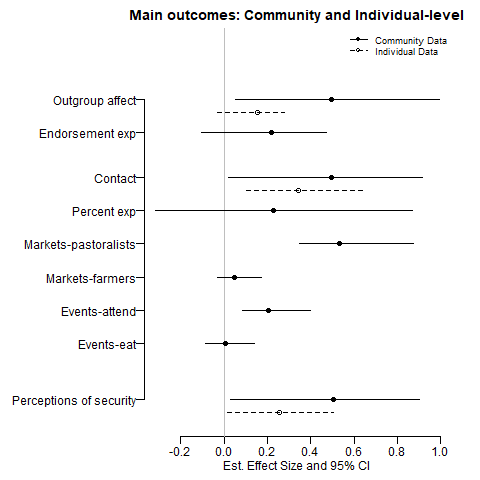
\includegraphics[width=.7\textwidth]{../../../figs/ecpn_coefplots_MainOuts-cats.png}
\caption{\label{fig:fig1} \textbf{Effect of treatment assignment on outcomes in community-level and individual-level data.} Points are average treatment effects versus control estimated using OLS. Lines are bootstrapped 95\% confidence intervals.  Solid lines are effects in the community-level data, dashed lines are effects in the individual-level data.  The first set of effects concern intergroup affect; the second set concern voluntary contact; the last concerns insecurity.  Effects in the figure are positive if ECPN improved outcomes and negative if ECPN worsened outcomes.}
\end{figure}

Figures \ref{fig:fig1} and \ref{fig:fig2} shows ECPN's effect on all
primary outcomes. Figure 1 shows the main analyses, where the solid
lines are the community-level data and the dashed lines are the
individual-level data. Figure 2 shows participants and nonparticipants
compared to controls. From top to bottom, the outcomes are ordered to
correspond with: (1) intergroup attitudes, (2) intergroup contact, and
(3) insecurity. Some outcomes -- observations in markets and at social
events, survey experiments -- are only possible in the community-level
analysis.

\begin{figure}[H]
\centering
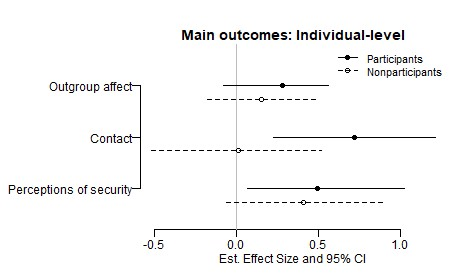
\includegraphics[width=.7\textwidth]{../../../figs/ecpn_coefplots_MainOuts_panel-cats2.jpg}
\caption{\label{fig:fig2} \textbf{Effect of treatment assignment on participants and nonparticipants.} Points are average treatment effects versus control estimated using OLS. Lines are bootstrapped 95\% confidence intervals.  Solid lines are effects among participants, dashed lines are effects among nonparticipants living in treatment communities.  Effects in the figure are positive if ECPN improved outcomes and negative if ECPN worsened outcomes.}
\end{figure}

\hypertarget{intergroup-affect}{%
\subsection{Intergroup Affect}\label{intergroup-affect}}

ECPN bolstered intergroup affect in treatment communities. Compared to
control communities, respondents in treatment communities report more
trust in the other group and are more comfortable engaging in various
relationships with the outgroup, such as trading goods and
intermarriage. Intergroup affect as measured by the endorsement
experiment also improves more in the treatment group than the control
group, though the difference is not statistically significant at
conventional levels.

Figures \ref{fig:fig3} and \ref{fig:fig4} show the descriptive change in
affect for treatment and control communities. Affect in control
communities decreased from baseline to endline, while intervention
communities improved over the same time period. As measured by the
endorsement experiment, affect declines in both treatment and control
communities, but declines more in control communities. Both measures
suggest that ECPN improved affect towards the outgroup.

\begin{figure}[H]
    \begin{subfigure}[b]{.48\textwidth}
    \centering
        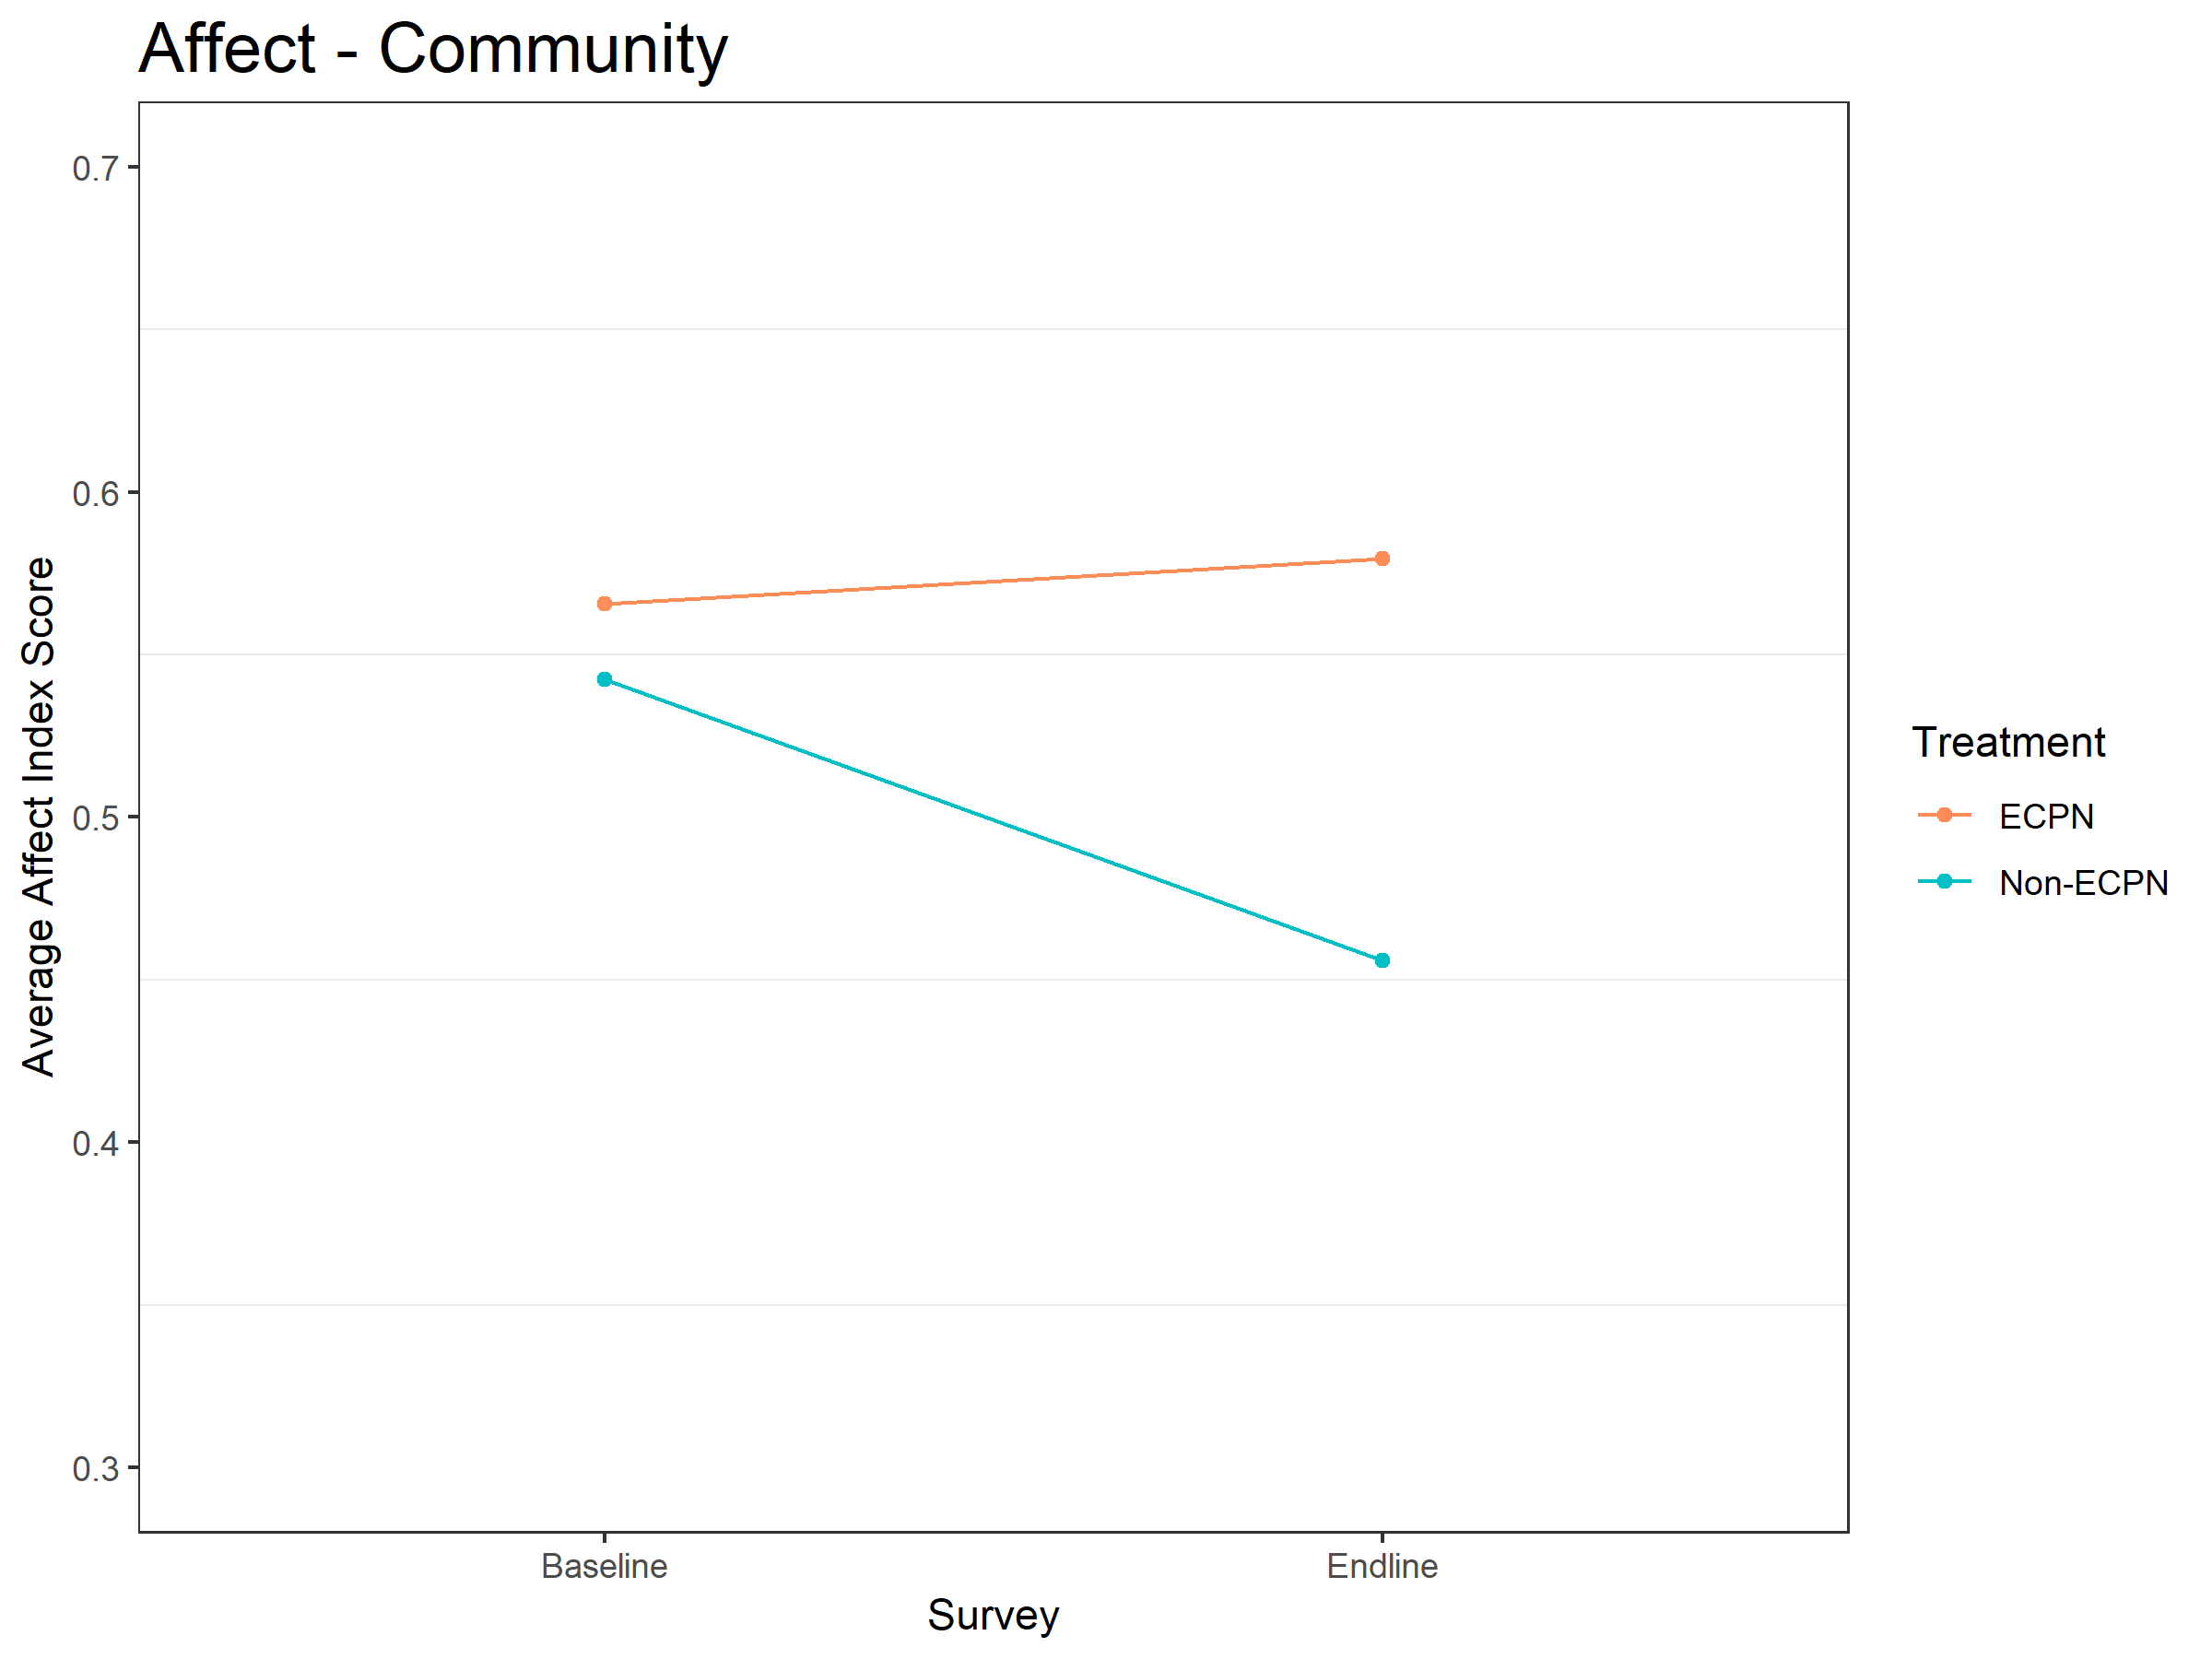
\includegraphics[width=\linewidth]{../../../figs/affectComm_plot.png}
        \caption{\textbf{Descriptive change in community-level intergroup affect from baseline to endline.} Red line is treatment site average, blue line is control site average.  Moving up the Y-axis indicates improved affect between groups.}
        \label{fig:fig3}
    \end{subfigure}
    \hfill
    \begin{subfigure}[b]{.48\textwidth}
    \centering
        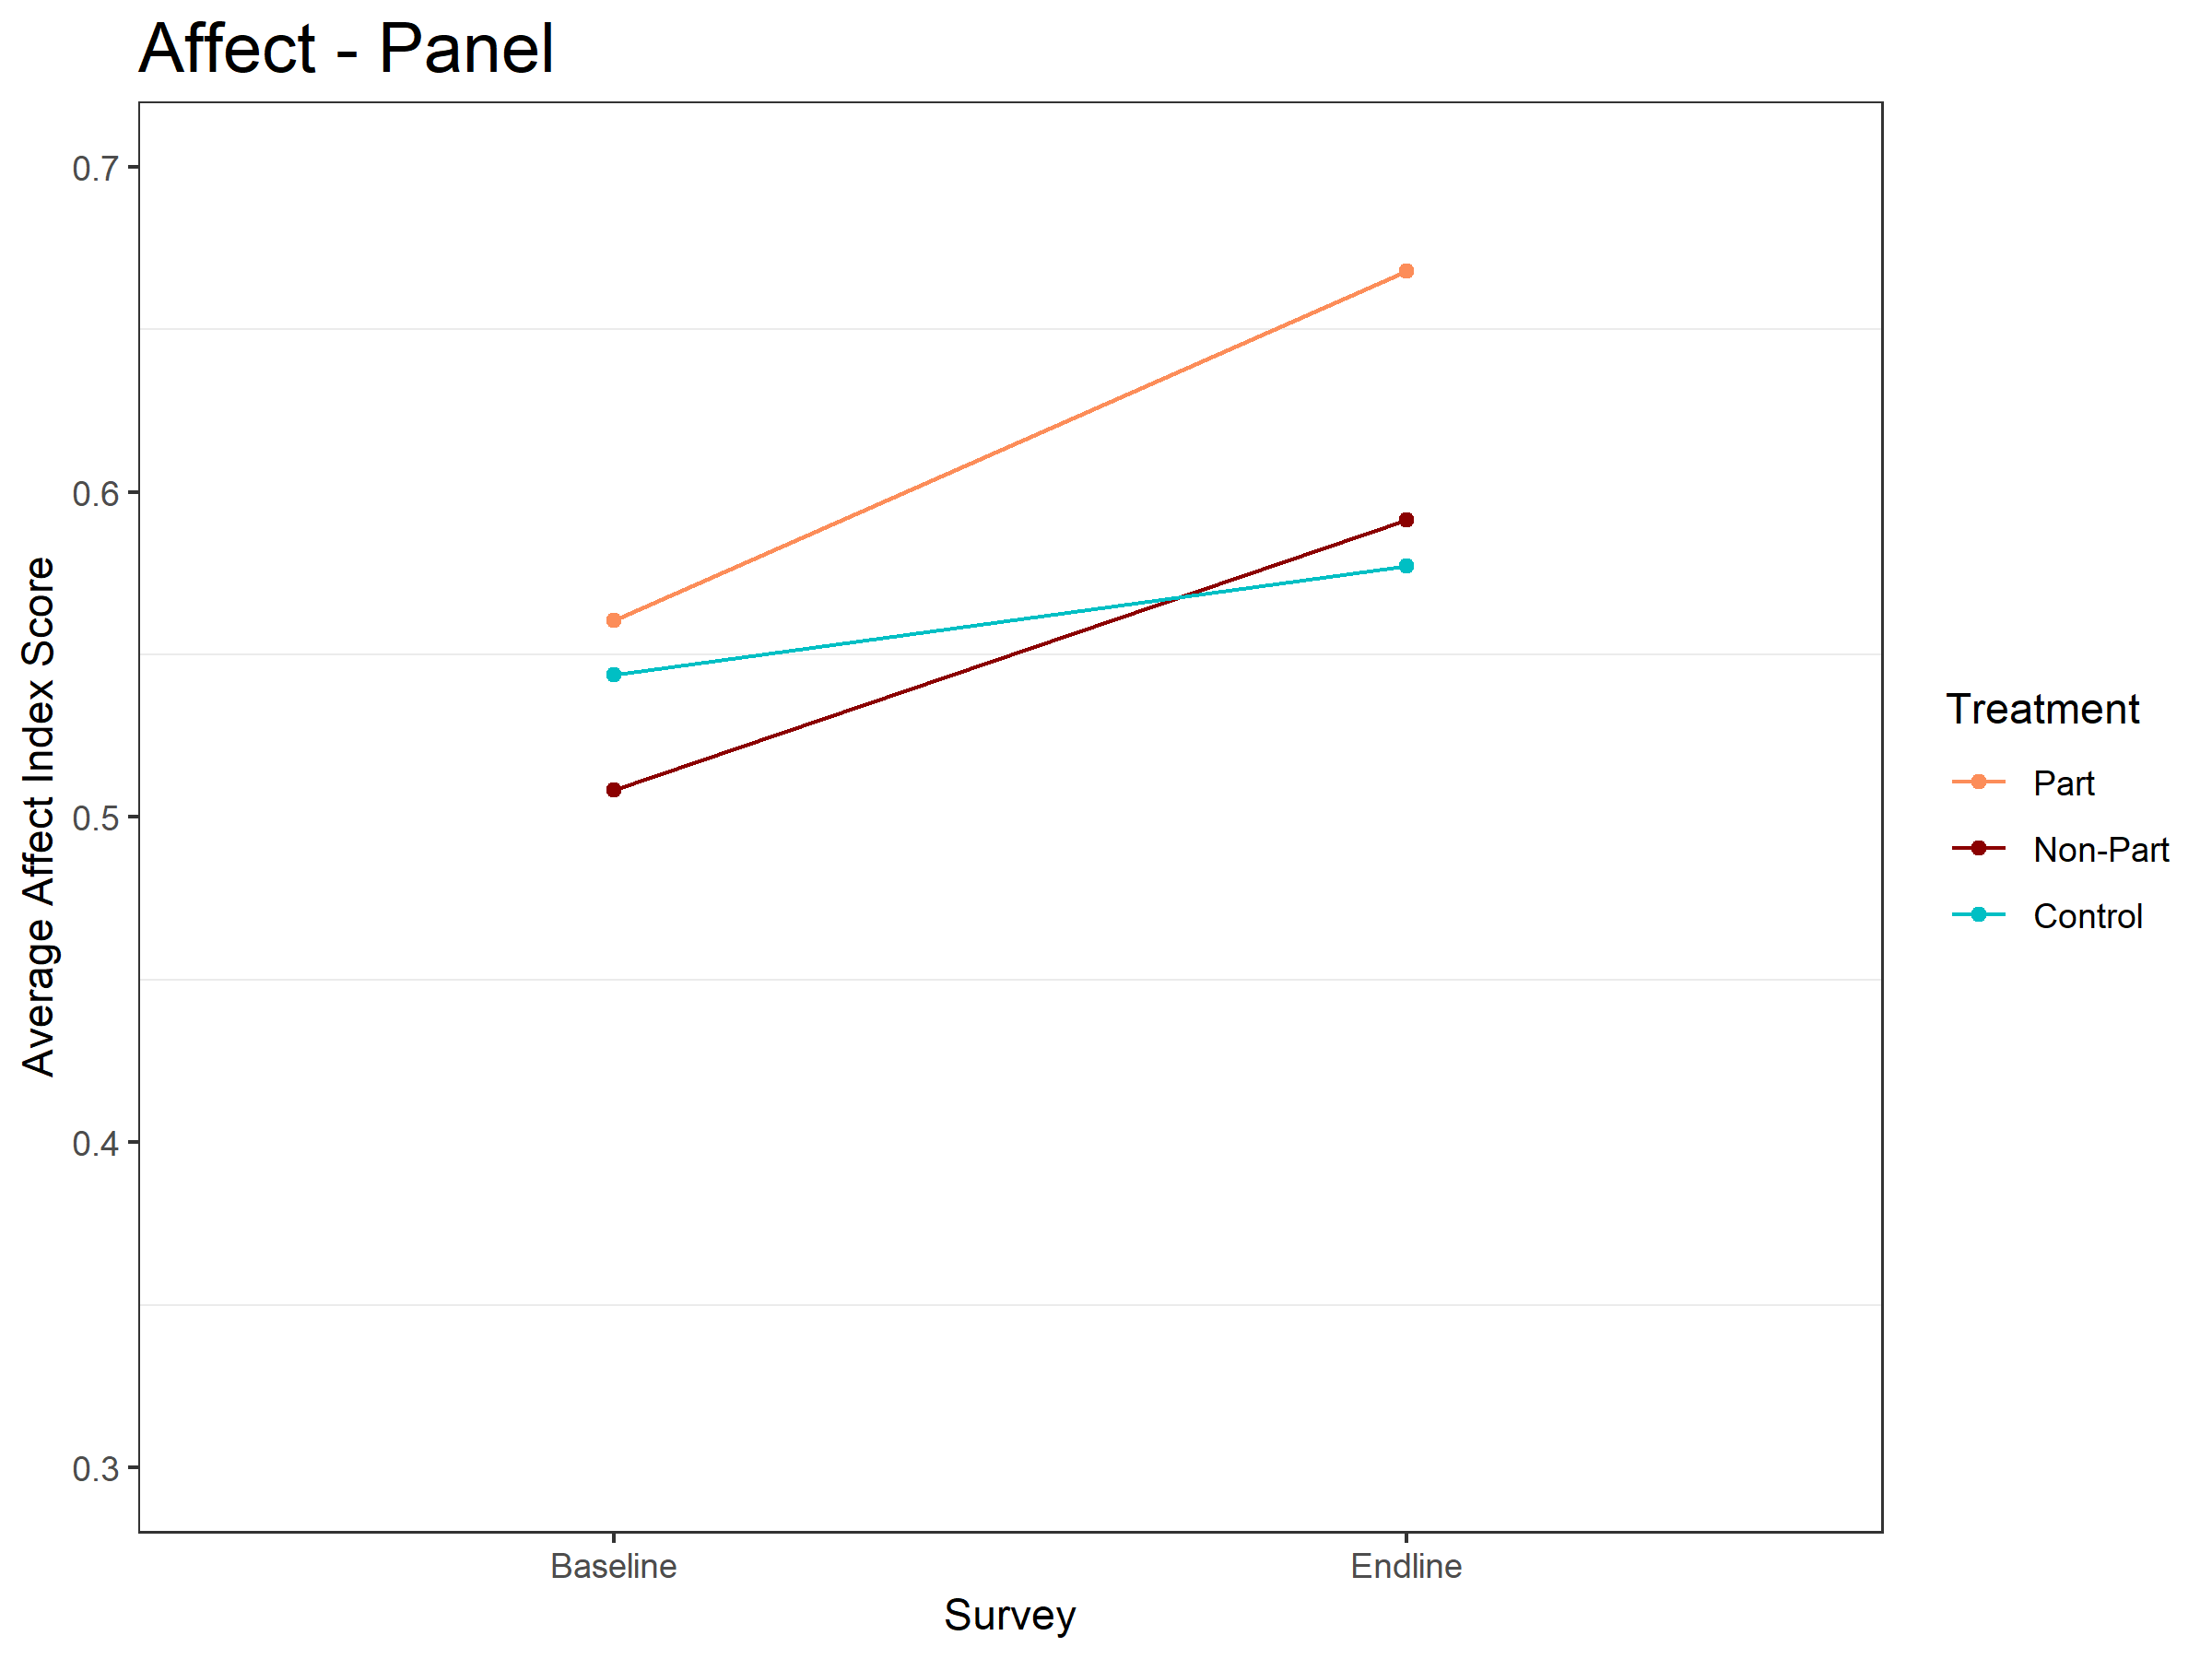
\includegraphics[width=\linewidth]{../../../figs/affectPan_plot.png}
        \caption{\textbf{Descriptive change in individual-level intergroup affect from baseline to endline.} Red line is participant average, dark red line is nonparticipant average, blue line is control average.}
        \label{fig:fig4}
    \end{subfigure}
\caption{Intergroup Affect}
\end{figure}

\hypertarget{contact}{%
\subsection{Contact}\label{contact}}

The effect of ECPN on contact is substantial. Respondents in treatment
communities report more contact and more willingness to engage in
contact at all levels of the percent experiment; we also observe more
pastoralists in markets interacting with farmers. Since the markets are
all located in the farming community, the sustained presence of
pastoralists there suggests that (1) farmers were accepting/tolerant of
pastoralists in their community and (2) pastoralists felt comfortable
spending time in the farmer community. The number of farmers present in
the markets does not change in either group, which makes sense because
the market is inside the farming community.

\begin{figure}[H]
    \begin{subfigure}[b]{.48\textwidth}
    \centering
        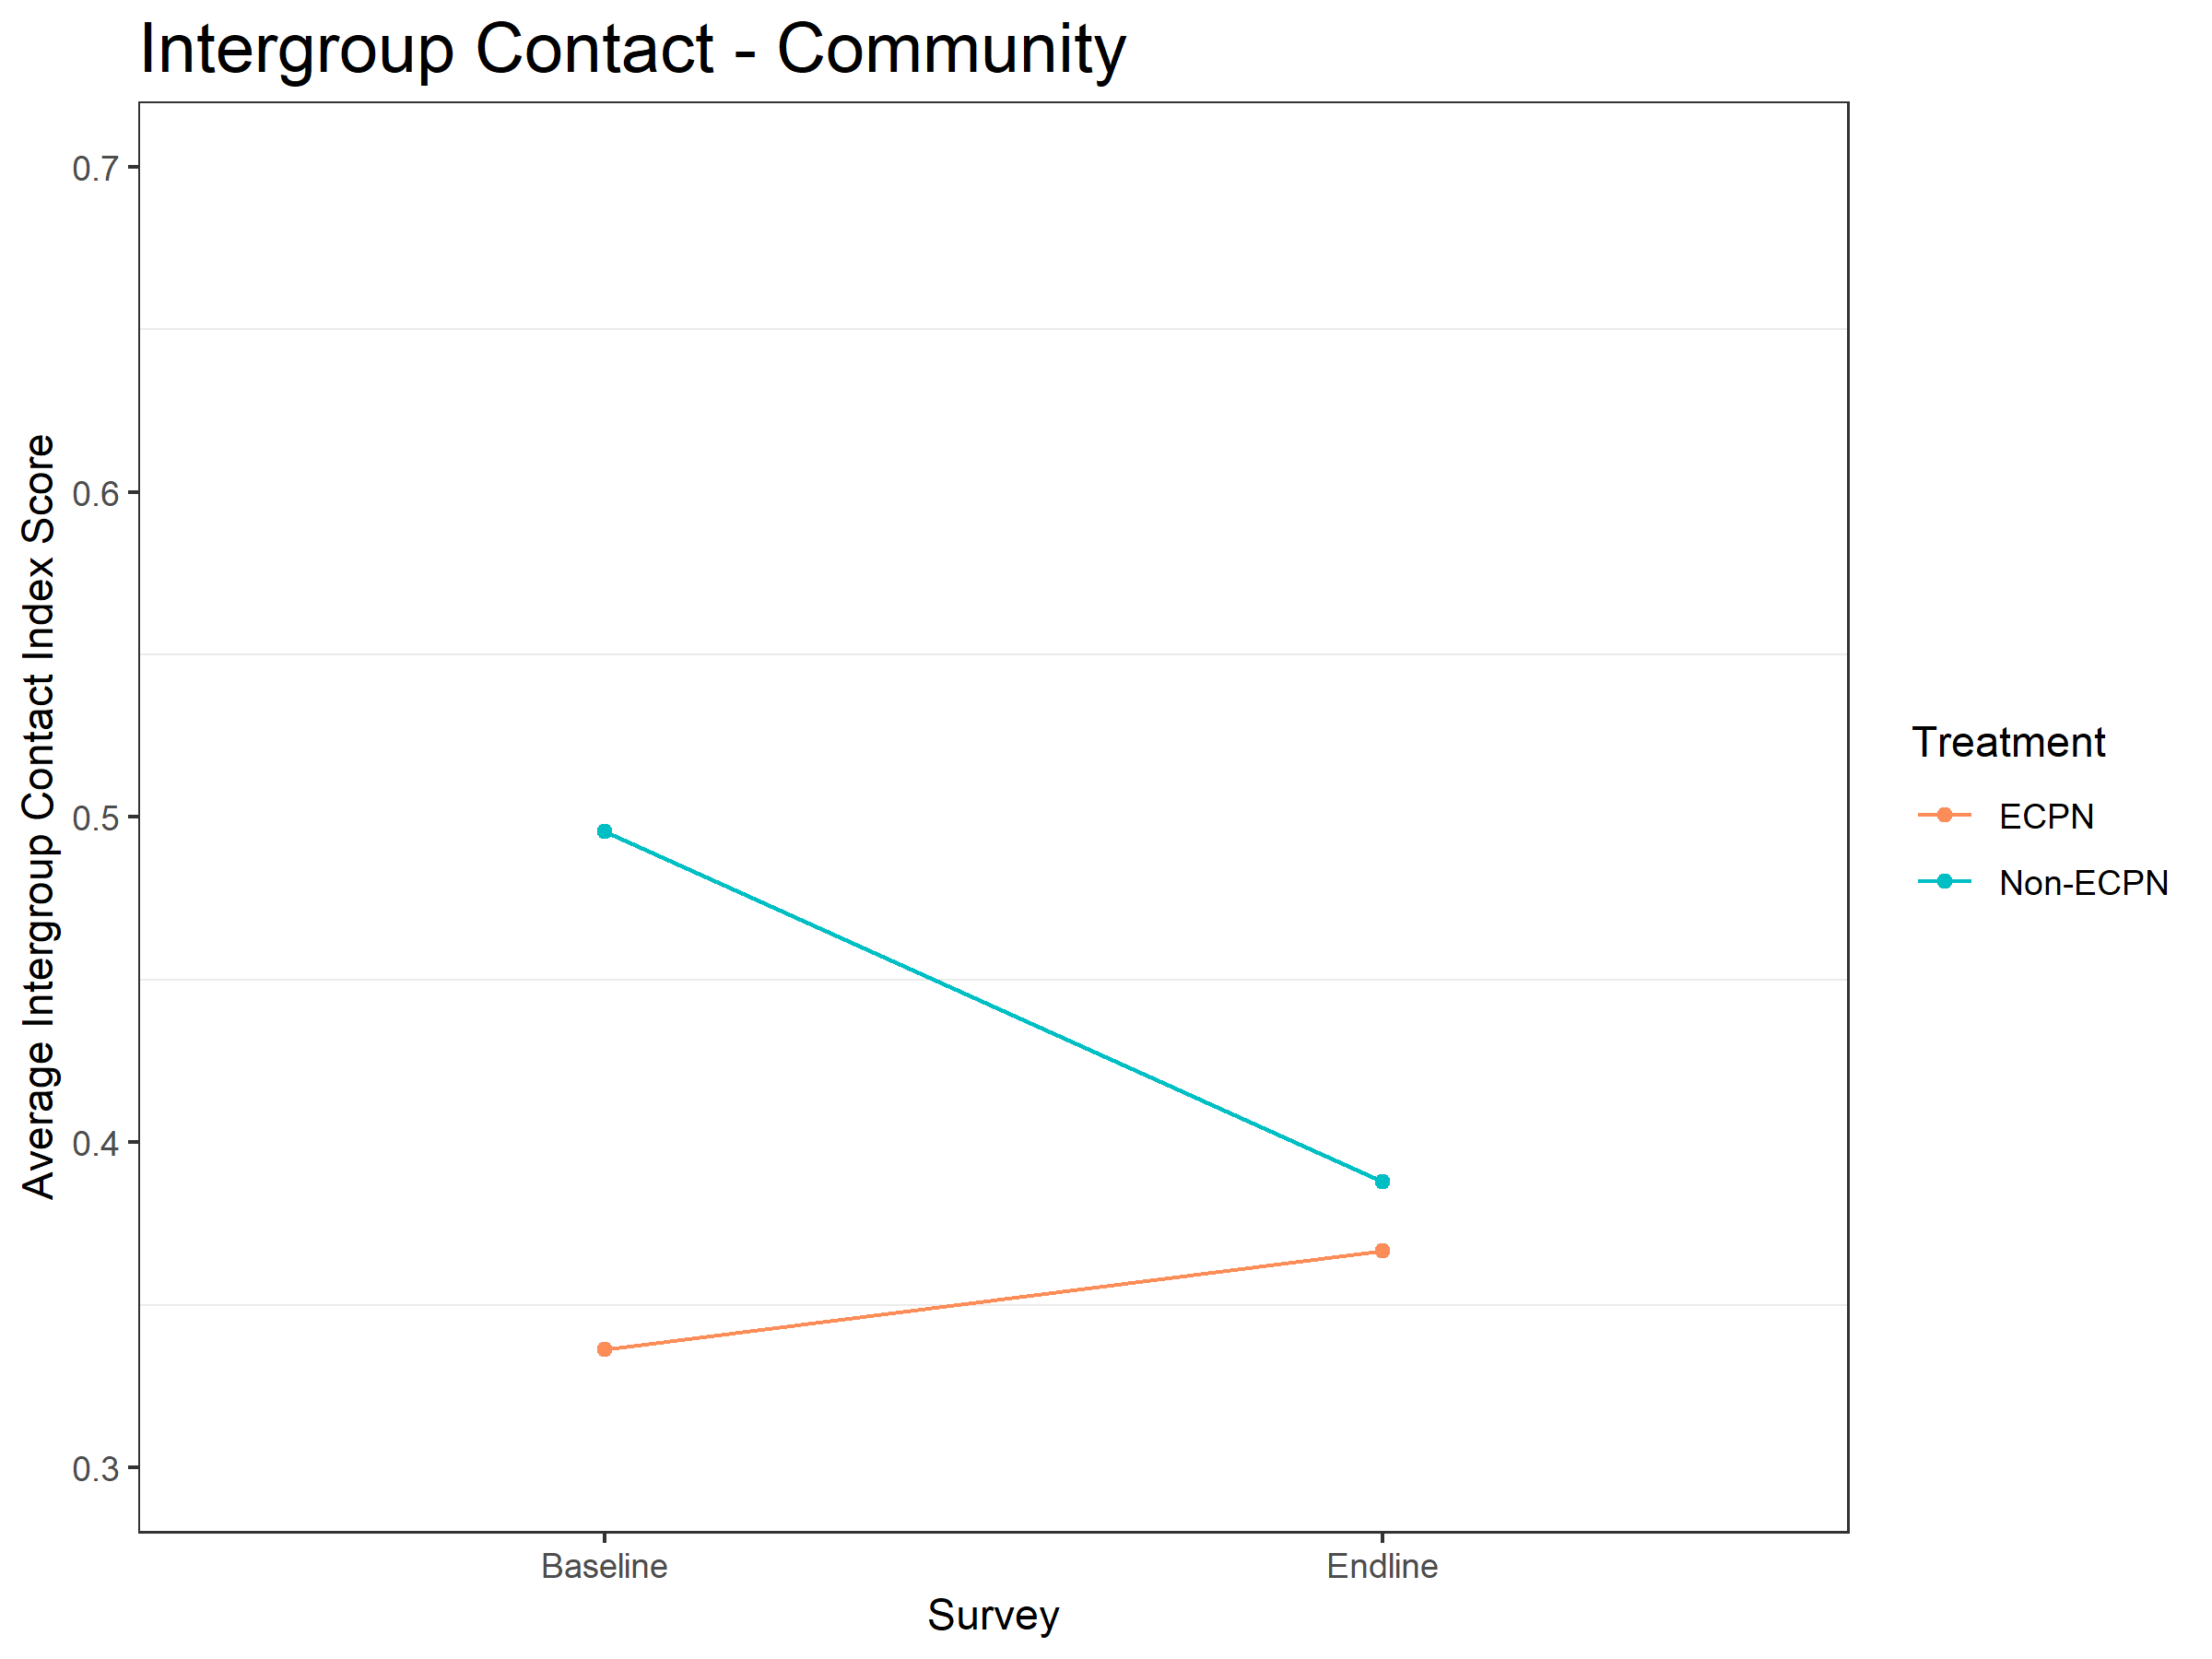
\includegraphics[width=\linewidth]{../../../figs/conComm_plot.png}
        \caption{\textbf{Descriptive change in community-level voluntary contact from baseline to endline.} Red line is treatment site average, blue line is control site average.  Moving up the Y-axis indicates improved affect between groups.}
        \label{fig:fig5}
    \end{subfigure}
    \hfill
    \begin{subfigure}[b]{.48\textwidth}
    \centering
        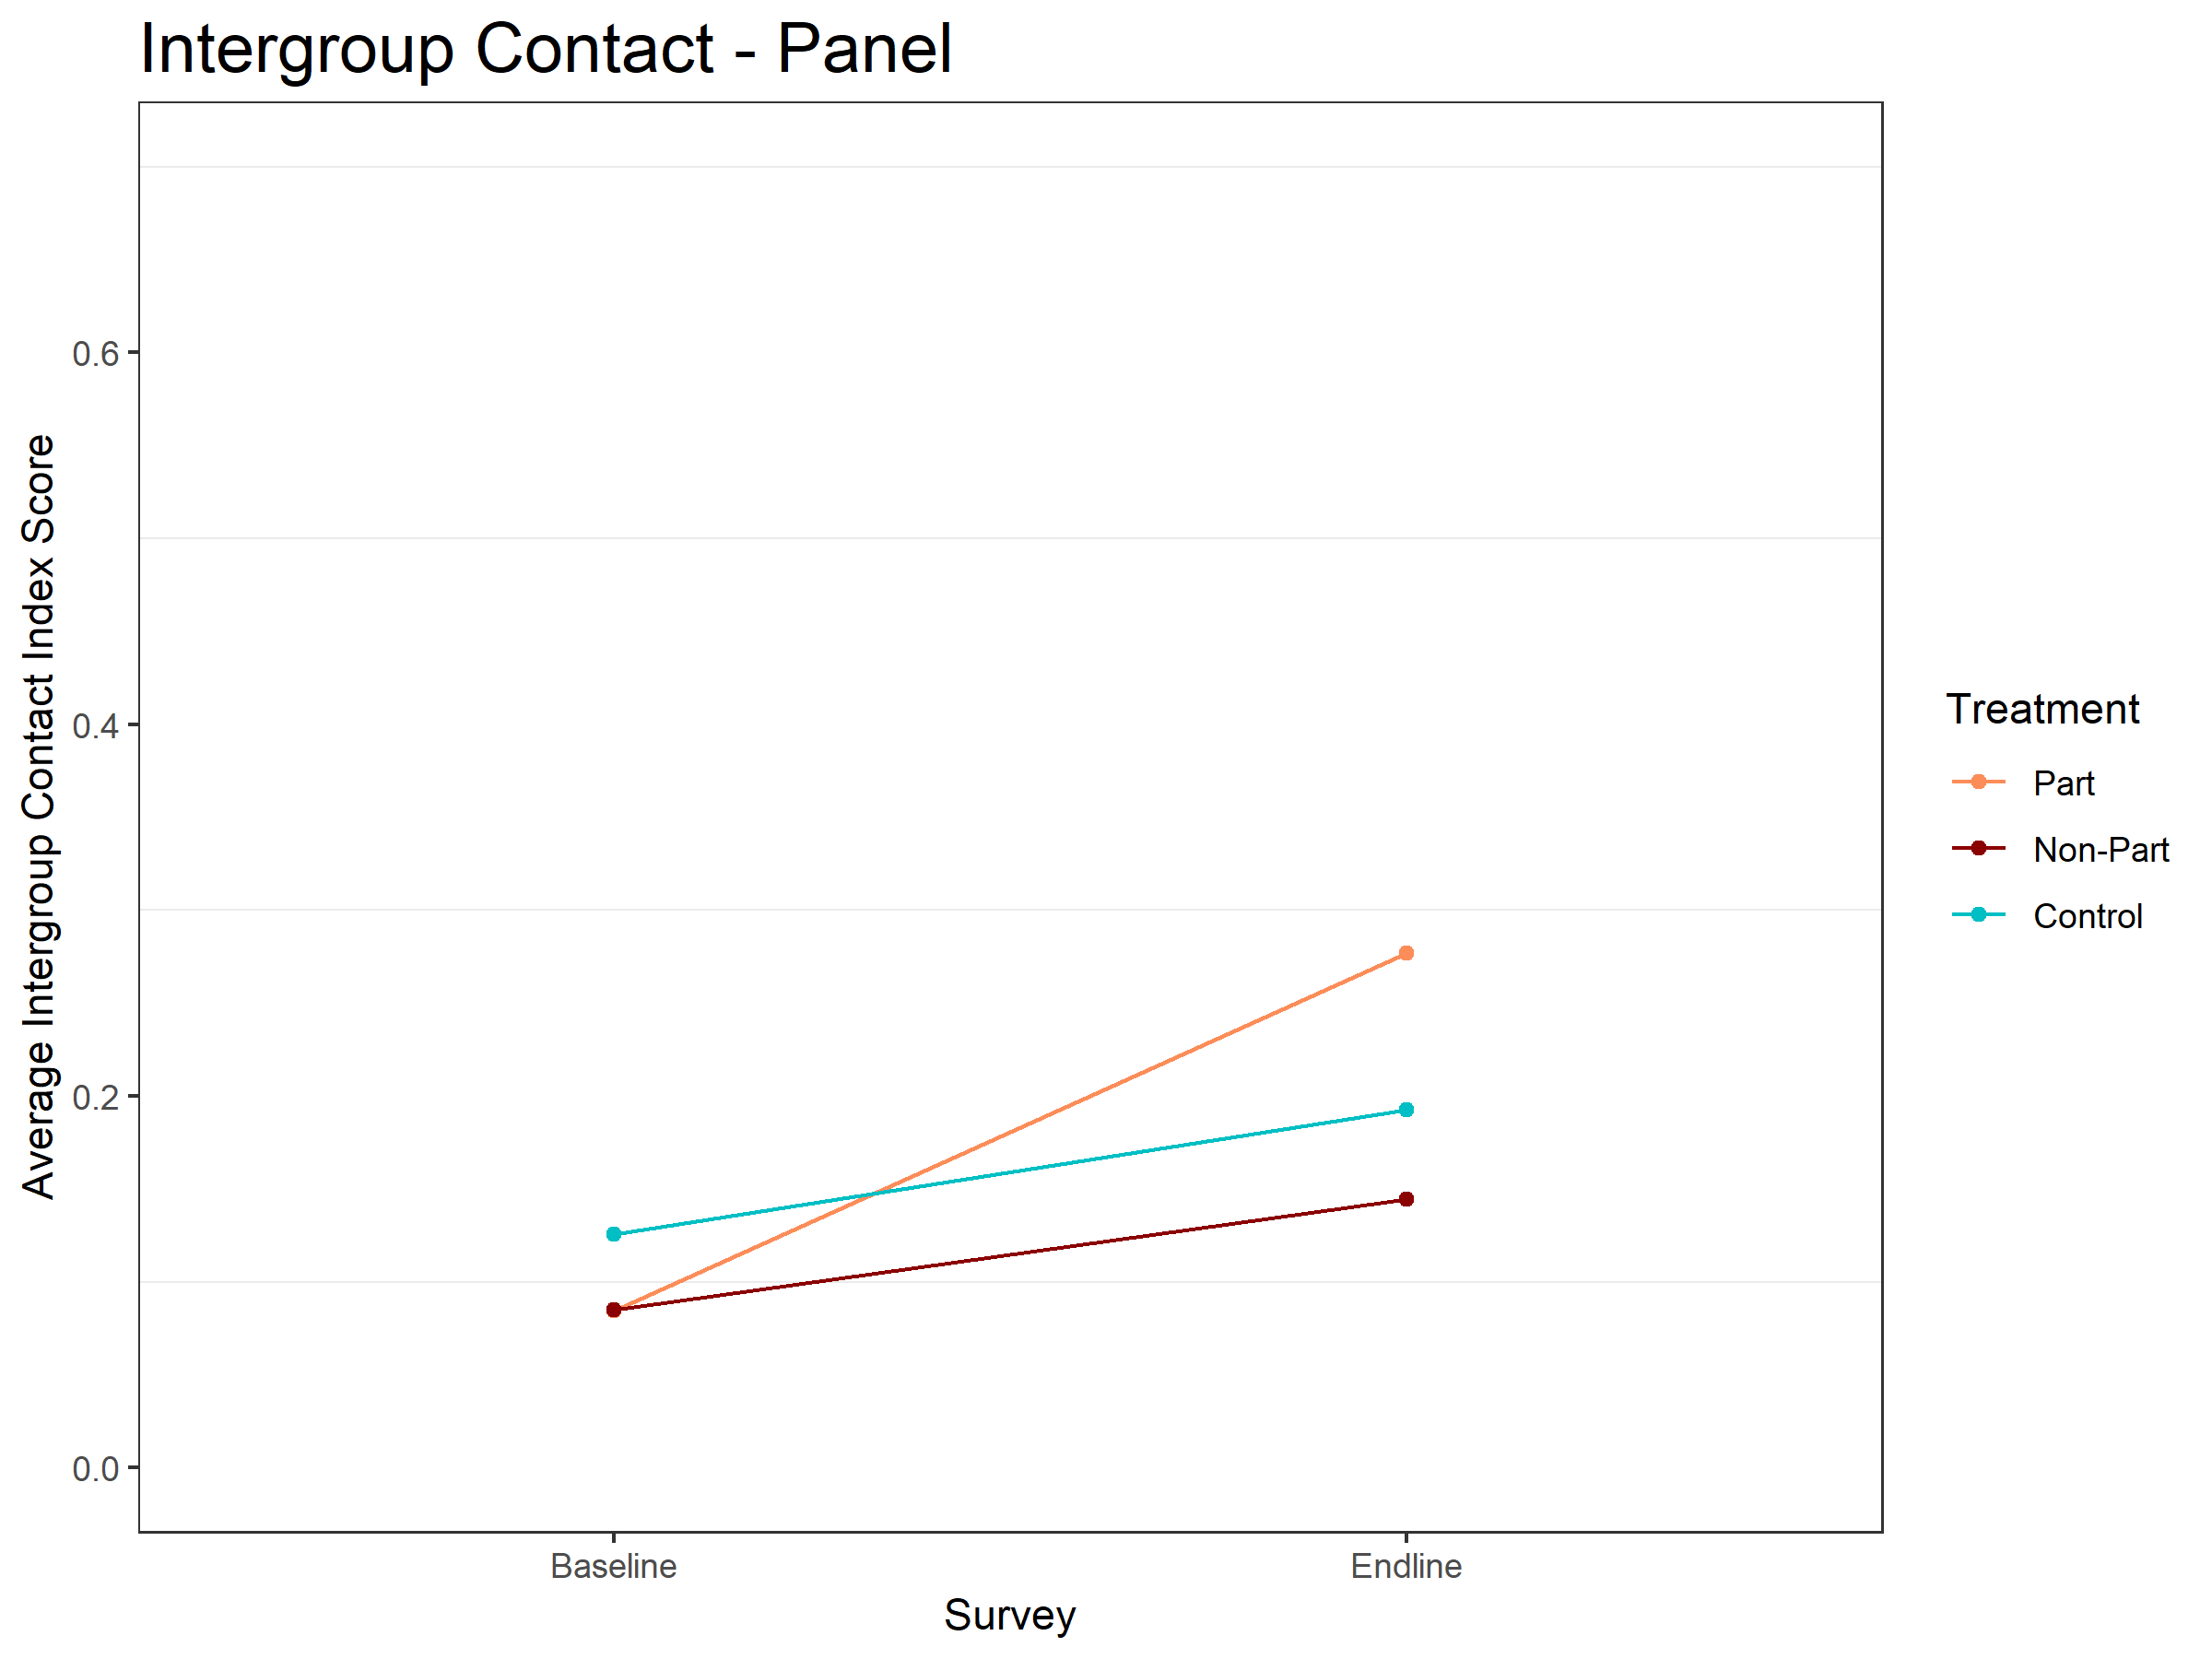
\includegraphics[width=\linewidth]{../../../figs/conPan_plot.png}
        \caption{\textbf{Descriptive change in individual-level voluntary contact from baseline to endline.} Red line is participant average, dark red line is nonparticipant average, blue line is control average.}
        \label{fig:fig6}
    \end{subfigure}
    \caption{Voluntary Contact}
\end{figure}

Figures \ref{fig:fig5} and \ref{fig:fig6} show the descriptive change in
contact for treatment and control communities. The community-level
self-reports show that intergroup contact declined sharply in control
communities but rose slightly in treatment communities. It is impressive
that ECPN increased contact while the social environment led to a sharp
decline in control sites. The secular decline is due to the displacement
in Benue, where intergroup contact went down for every group, though it
declined far less in treatment sites. In Nassarawa, intergroup contact
increased in both treatment and control sites, but far more in treatment
sites.

At the individual-level, intergroup contact increased for committee
participants but stayed largely the same for nonparticipants and
controls. The large community-level effect, however, suggests that the
effects of ECPN \emph{did} extend to nonparticipants in treatment
communities. But the effect did not extend to the type of nonparticipant
who we could track down and resurvey.

\hypertarget{insecurity}{%
\subsection{Insecurity}\label{insecurity}}

ECPN's substantially decreased feelings of insecurity in the treatment
group. The effect is large in both the community-level and the
individual-level data. Security in ECPN communities improved far more
from baseline to endline than in control communities. At the
individual-level, participants and nonparticipants improved equally,
suggesting that these increases reflect a change in the conflict
environment that impacts the entire community, not just respondents
involved in ECPN committees. These improvements in treatment communities
are especially powerful because other survey questions show that ECPN
increased awareness of the conflict -- respondents in ECPN communities
are more likely than the control to know that violence between groups
has occurred recently, yet they feel more secure.

\begin{figure}[H]
    \begin{subfigure}[b]{.48\textwidth}
    \centering
        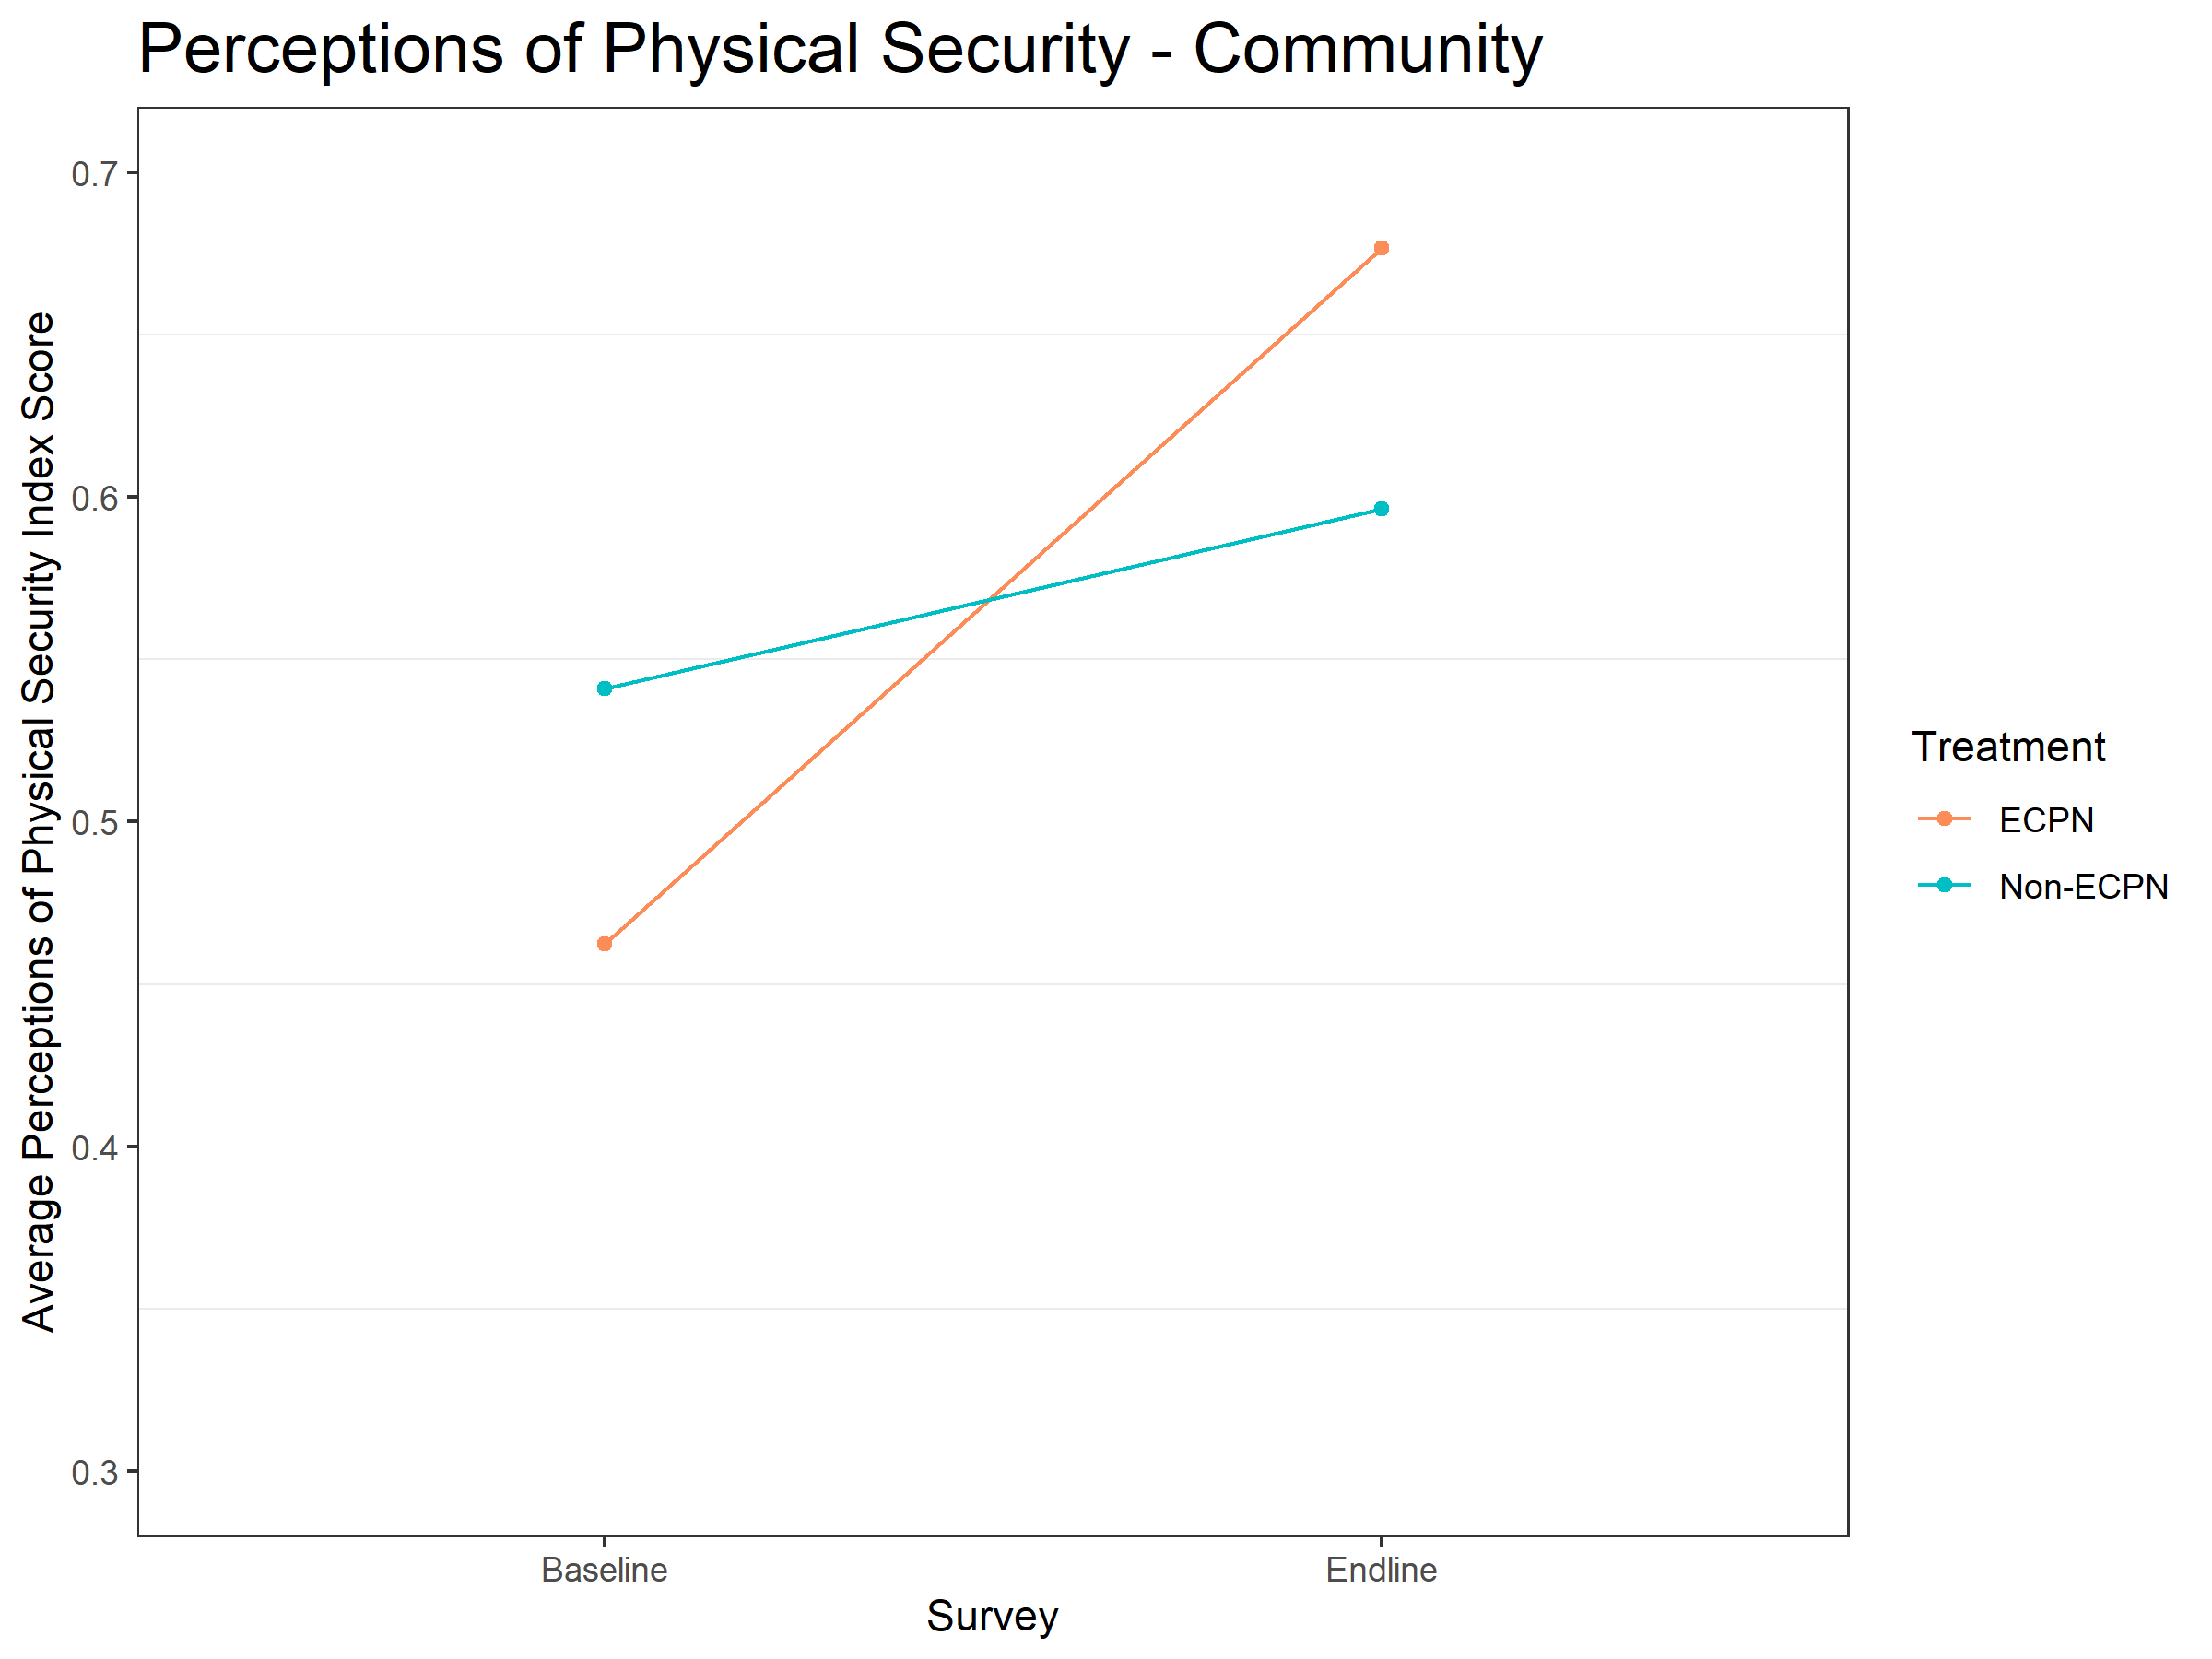
\includegraphics[width=\linewidth]{../../../figs/inComm_plot.png}
        \caption{\textbf{Descriptive change in community-level insecurity from baseline to endline.} Red line is treatment site average, blue line is control site average.  Moving up the Y-axis indicates improved affect between groups.}
        \label{fig:fig7}
    \end{subfigure}
    \hfill
    \begin{subfigure}[b]{.48\textwidth}
    \centering
        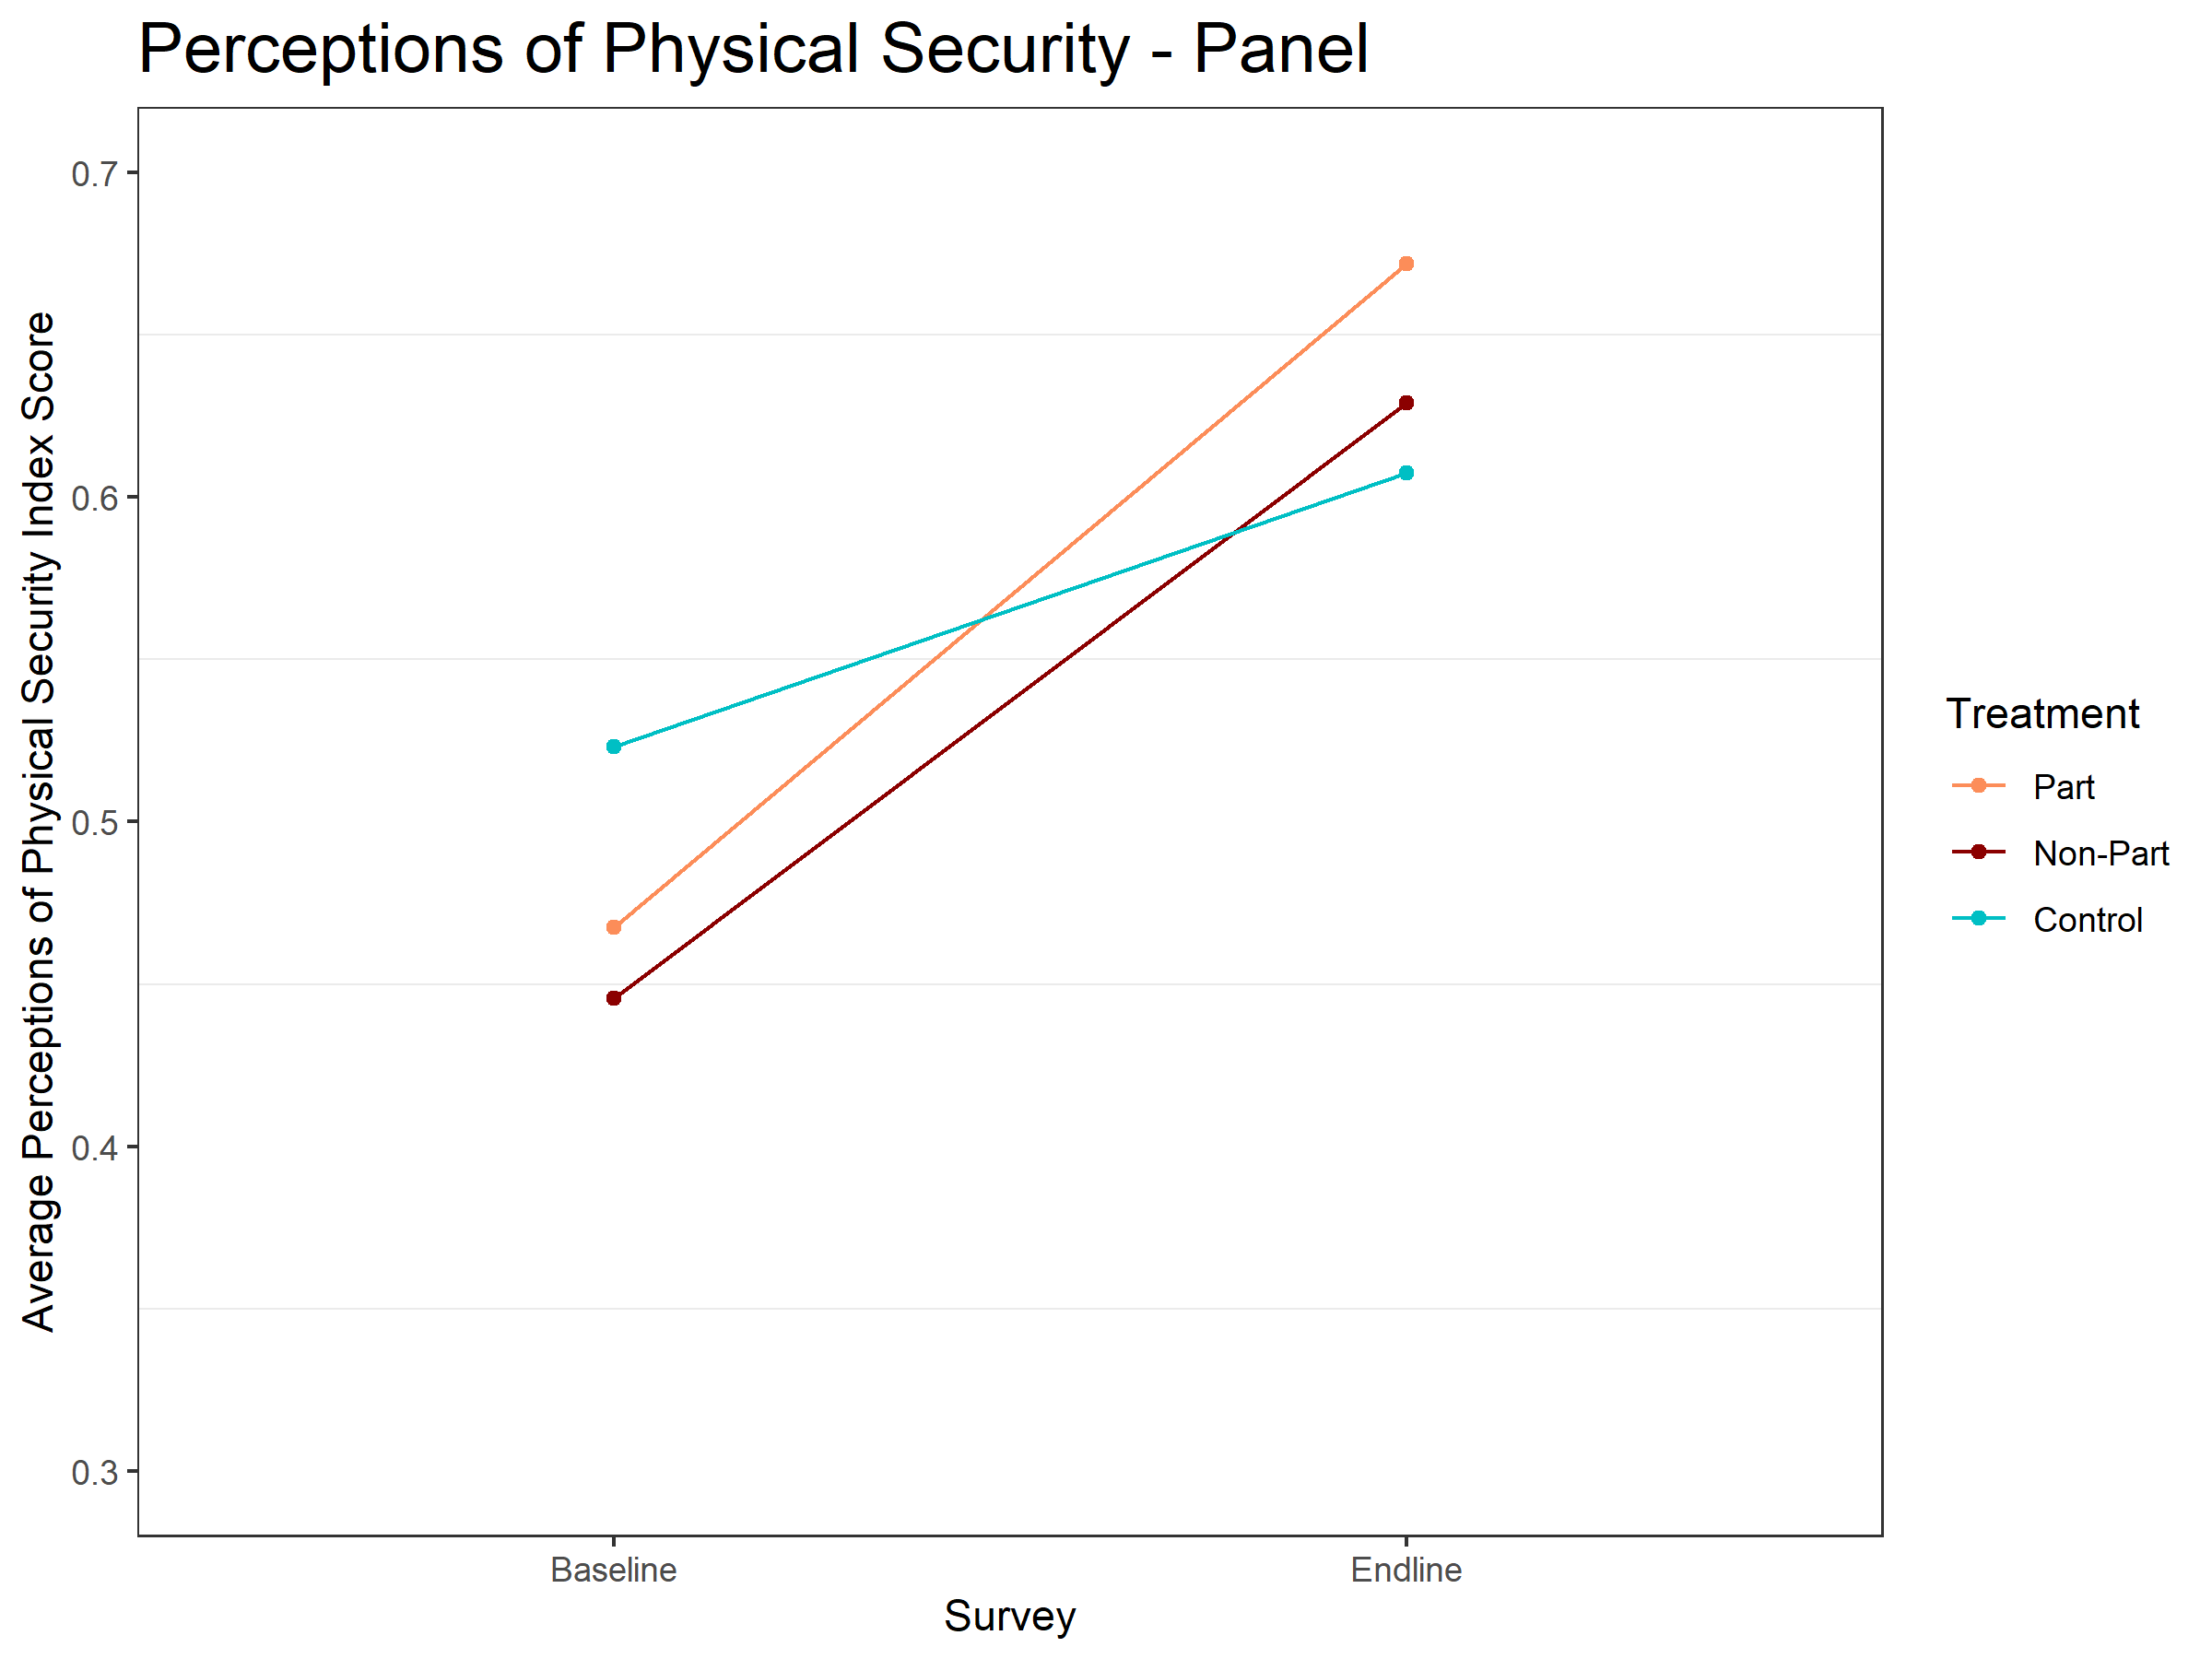
\includegraphics[width=\linewidth]{../../../figs/inPan_plot.png}
        \caption{\textbf{Descriptive change in individual-level insecurity from baseline to endline.} Red line is participant average, dark red line is nonparticipant average, blue line is control average.}
        \label{fig:fig8}
    \end{subfigure}
    \caption{Voluntary Contact}
\end{figure}

Figures \ref{fig:fig7} and \ref{fig:fig8} show the descriptive change in
insecurity for treatment and control communities. The insecurity of
control communities declines slightly from baseline to endline but
insecurity in treatment communities declines substantially more. ECPN
communities initially felt more insecure than control communities but
were more secure at the end of the program. ECPN substantially improved
the security of people in intervention communities.

\hypertarget{placebo-attitudes-about-violence}{%
\subsection{Placebo: attitudes about
violence}\label{placebo-attitudes-about-violence}}

To provide evidence that these survey results are due to intergroup
contact and not due to social desirability bias, we analyze the effect
of ECPN on attitudes about violence. If ECPN affects attitudes about
violence, then we worry that other self-reports were affected by social
desirability bias. If ECPN has no effect on attitudes about violence,
then it is unlikely that other self-reports were affected by social
desirability bias.

ECPN has no effect on attitudes about violence in the community-level
data or the individual-level data. The lack of an effect on this placebo
outcome, plus our use of survey experiments and behavioral observation
to corroborate survey self-reports, suggests that our self-report
results for primary outcomes are not due to social desirability bias.
More details about the placebo analysis are available in Appendix C.

\hypertarget{mechanisms-empathy-threat-and-ingroup-expansion}{%
\subsection{Mechanisms: Empathy, Threat, and Ingroup
Expansion}\label{mechanisms-empathy-threat-and-ingroup-expansion}}

Our results suggest that ECPN improved intergroup relations between
farmers and pastoralists. We also undertook an exploratory analysis to
learn the mechanisms through which ECPN affected attitudes. Based on the
literature about contact theory, we looked for evidence that ECPN worked
through empathy and perspective-taking, reduced feelings of threat, and
expansion of the respondent's ingroup to include the former outgroup.

Our exploratory analysis suggests that ECPN may have worked through
increasing empathy. ECPN led to increased empathy in the community and
individual-level analyses. In turn, increased empathy correlated with
improved intergroup affect in the community-level data and with
increases in intergroup affect and intergroup contact at the individual
level. Increased perspective-taking also correlated with intergroup
affect and intergroup contact in both analyses. ECPN may have led to
increased perspective-taking, though not quite to a statistically
significant level. This analysis suggests that increased empathy is a
plausible mechanism through which ECPN improved intergroup relations.
Because empathy was not randomly assigned, though, it's equally
plausible that ECPN improved intergroup affect and fostered intergroup
contact, and that those outcomes led to increased empathy.

There is no evidence that ECPN reduced perceptions of threat or expanded
perceptions of the ingroup. ECPN did not effect either survey index, and
the public goods game shows that the treatment group was not better at
coordinating than the control group. Treatment communities donated
\emph{less} to the shared community fund than control communities. At
the individual-level, ECPN participants donated less than
nonparticipants who donated less than respondents in the control group.
This is the opposite pattern of what we would expect if intergroup
contact caused the communities to think of each other as part of one
ingroup. Reduced threat and ingroup expansion are still plausible
psychological mechanisms -- each correlated strongly with at least one
outcome -- though neither was increased by ECPN.

More details about the mechanisms analyses can be found in Appendix C.

\hypertarget{discussion}{%
\section{Discussion}\label{discussion}}

This paper provides evidence that intergroup contact can improve
intergroup relations, even in dire circumstances. We tested the effects
of a programmatic contact intervention in an active and escalating
conflict between farmers and pastoralists in Nigeria. The extreme
violence of this context and personal involvement of the research
subjects poses a tough test for contact to improve intergroup relations.
The violence provides grievances that feed outgroup animosity and
reinforce group differences, strengthen social and psychological
barriers to improving attitudes, and reinforces the perception that
groups' material incentives are opposed. Despite the difficult context,
the program improved intergroup affect, fostered more intergroup
contact, and decreased feelings of insecurity in these communities.
Methodologically, this study demonstrates the benefits of measuring
outcomes at baseline and endline in a treatment group and in a control
group as a means of capturing the secular trend.

We believe the program improved group relations and the prospects for
peace because groups shared a latent interest that could be activated by
contact. The shared interest was ``latent'' because it was not being
identified by the groups in conflict. Cooperative contact helped reveal
the latent shared interest to both groups by demonstrating how the
groups can work together to achieve a common goal and removing
psychological and social barriers to identifying the shared interest.
Contact also provides the groups with opportunities to send costly
signals of their intent to cooperate, which are important for intergroup
cooperation (Kydd 2000). More studies need to be conducted to determine
the limits of contact and the conditions under which contact can
effectively improve intergroup relations.

This study also points to an opportunity for collaboration between
scholars of intergroup contact and scholars of conflict. These
literatures are often concerned with the same end goal -- reducing
conflict -- but rarely speak to one another. Conflict scholars often see
conflict as a bargaining problem, and violence as a bargaining failure.
The conflict literature points to a lack of trust as the primary cause
of conflict and usually posits a strong third party actor as necessary
to guarantee peace. Intergroup contact research hints that intergroup
contact can create cooperative norms and institutions that serve the
same function as a strong third party. Improving relations -- especially
improving trust -- through psychological interventions like intergroup
contact can help groups overcome commitment problems and reduce the
likelihood of violence.

Contact could help establish cooperative norms and institutions in a
number of ways. In our fieldwork, we see evidence that contact
strengthened existing conflict resolution structures, like leader
arbitration. The leadership of each group convene with the ``plaintiff''
and ``defendant'' to arbitrate cross-group disagreements, such as cows
caught grazing on farmland. Our research partners on the ground noted
that these structures became more effective in ECPN communities because
pastoralists became more aware of the financial value of the crops
destroyed by cows and farmers became more aware of the difficulty of
controlling and corralling thousands of cows.\footnote{We are especially
  grateful to Israel Okpe for his observations about farmer-pastoralist
  conflict dynamics.} Contact could also encourage ingroup policing:
ingroup members punishing other ingroup members who violate the rights
of outgroup members (Ditlmann and Samii 2016; Fearon and Laitin 1996).
If groups ``punish {[}their own{]} miscreants'' (Fearon and Laitin 1996,
722), in a way that is visible to the other side, then the other side
does not need to retaliate against the
transgression.{[}\^{}ingroupPolice{]} Visible ingroup policing shows
each side that the other can be trusted, alleviating commitment
problems.

This paper also teaches us about settling disputes between sedentary
peoples and semi-nomadic peoples. Violent conflict between settled
peoples and semi-nomadic peoples is on the rise throughout Africa
(Kuusaana and Bukari 2015; Mwamfupe 2015; Nnoko-Mewanu 2018). This study
focuses on the Fulani, the largest semi-nomadic people on Earth
(Encyclopedia 2017). Their way of life makes them targets for violence
throughout Africa. Along with this conflict in Nigeria, Fulani in Mali
have been the targets of violence so severe that researchers at Armed
Conflict Location \& Event Data Project called it ``ethnic cleansing''
(Economist 2019). Understanding how to prevent violent conflict between
Fulani and settled peoples can help prevent violence that targets other
nomadic, semi-nomadic, and itinerant peoples, such as the Tuaregs in
West Africa, Kochi in Afghanistan, Khoisan of Southern Africa, and
Romani of Europe. Preventing such violence could help preserve a dying
way of life.

There remain several opportunities to learn about the effects of contact
in conflict environments. First, this study employed a design to test
the hypothesis that contact would improve group relations in an active
conflict. It also provided exploratory evidence of the mechanisms
through which contact affects group relations, showing that contact may
have worked through increased empathy. Future studies can bring more
causal evidence to the question of \emph{how} contact improves group
relations. Second, our program was designed, implemented, and randomized
at the community-level because conflict between farmers and pastoralists
occurs at the community level. Future studies should randomize
individual community members' participation in a contact-based
intervention. Such studies could learn much about the affect of contact
on individuals, including the dosage of contact necessary to improve
attitudes, as well as how social norms and interpersonal discussion
diffuse the positive effects of contact to individuals without outgroup
contact.

Third, contact interventions, explicitly or implicitly, involve the
groups cooperating to \emph{achieve} a joint goal. ECPN was designed to
benefit all communities by having the conflicting communities cooperate
successfully. But what if contact is not successful and the goal is not
achieved? Does contact itself still improve attitudes, or does contact
work because groups begin to associate cross-group cooperation with good
outcomes? In a similar vein, are Allport's conditions necessary for
contact to achieve its aims, or are they only needed insofar as they
ensure the intergroup cooperation generates positive outcomes for both
groups? Future studies should determine the necessity of Allport's
conditions and attempt to differentiate the fact of contact from the
outcomes that group cooperation produces.

\hypertarget{appendices}{%
\section{Appendices}\label{appendices}}

\hypertarget{appendix-a-randomization-inference-and-bootstrapping}{%
\subsection{Appendix A: Randomization Inference and
Bootstrapping}\label{appendix-a-randomization-inference-and-bootstrapping}}

Randomization inference and bootstrapping are nonparametric methods to
generate \(p\)-values (randomization inference) and confidence intervals
(bootstrapping). With \emph{randomization inference}, we first shuffle
the treatment variable to break the relationship between treatment and
outcomes. Next we regress outcomes on treatment using our regression
equation and store the resulting coefficient. Lastly, we repeat that
process 10,000 times to create the distribution of coefficients we would
observe if treatment had no effect on outcomes -- the null hypothesis.
Our \(p\)-value is the proportion of the null distribution that is
greater than or equal to our observed coefficient.

\emph{Bootstrapping} for standard errors is similar, but instead of
shuffling the treatment indicator we resample units with replacement. By
resampling with replacement, we create the empirical distribution of our
data and the range of possible treatment effects we might observe if we
repeated the experiment 10,000 times. The treatment effect at the 2.5th
percentile and at the 97.5th percentile are equivalent to a 95\%
confidence interval (Efron and Tibshirani 1994).

In each of these procedures, we mimic our randomization process by
randomizing/resampling the intervention to communities in site-level
clusters and within state blocks. This means that both communities in an
implementation site (farmers and pastoralists) will always be
treated/sampled together and that assignment to the intervention and
resampling are conducted separately in Nassarawa and Benue, just as the
intervention was assigned in this study. This procedure ensures that our
null distribution (for \(p\)-values) is created by randomizing the
intervention between exchangeable units and that our empirical
distribution (for confidence intervals) is created by resampling units
as they were sampled.

\hypertarget{appendix-b-results-with-additive-indices}{%
\subsection{Appendix B: Results with Additive
Indices}\label{appendix-b-results-with-additive-indices}}

These tables show results for self-report survey outcomes made with
additive indices. The tables include the coefficients and \(p\)-values
with additive indices for community- and individual-level analyses.

\begin{table}[H]
\begin{center}

\begin{tabular}{l|r|r|r|r}
\hline
  & ag\_coef & ag\_p & ind\_coef & ind\_p\\
\hline
Affect & 0.093 & 0.037 & 0.062 & 0.056\\
\hline
Insecurity & 0.015 & 0.174 & 0.030 & 0.011\\
\hline
Contact & 0.054 & 0.193 & 0.070 & 0.143\\
\hline
\end{tabular}


\caption{\label{tab:add_ind_tab}\textbf{Effect of ECPN on main outcomes with additive indices.} The first and second columns are coefficients and $p$-values for aggregate community-level analyses.  The third and fourth columns are coefficients and $p$-values for individual-level analyses.}
\end{center}
\end{table}

\hypertarget{appendix-c-mechanisms-and-placebo-analysis}{%
\subsection{Appendix C: Mechanisms and Placebo
Analysis}\label{appendix-c-mechanisms-and-placebo-analysis}}

These tables show results for mechanism and placebo outcomes using
inverse-covariance weighted indices. The tables include the coefficients
and \(p\)-values for community- and individual-level analyses.

\begin{table}[H]
\begin{center}

\begin{tabular}{l|r|r|r|r}
\hline
  & ag\_coef & ag\_p & ind\_coef & ind\_p\\
\hline
Threat & -0.065 & 0.796 & 0.007 & 0.350\\
\hline
Empathy & 0.129 & 0.089 & 0.127 & 0.010\\
\hline
Perspective-Taking & -0.040 & 0.640 & 0.029 & 0.195\\
\hline
Ingroup Expansion & 0.036 & 0.252 & 0.016 & 0.166\\
\hline
Placebo (Violence) & -0.067 & 0.691 & -0.007 & 0.556\\
\hline
\end{tabular}


\caption{\label{tab:mech_ind_tab}\textbf{Effect of ECPN on mechanism and placebo outcomes.} The first and second columns are coefficients and $p$-values for aggregate community-level analyses.  The third and fourth columns are coefficients and $p$-values for individual-level analyses.}
\end{center}
\end{table}

\hypertarget{appendix-d-survey-questions}{%
\subsection{Appendix D: Survey
Questions}\label{appendix-d-survey-questions}}

\textbf{Outgroup Affect}

\begin{itemize}
\tightlist
\item
  With regards to someone from {[}X GROUP{]}, would you feel
  comfortable:

  \begin{itemize}
  \tightlist
  \item
    if they worked in your field?
  \item
    paying them to watch your animals?
  \item
    trading goods with them?
  \item
    sharing a meal with them?
  \item
    with a close relative marrying a person from {[}X GROUP{]}?
  \end{itemize}
\item
  From 1-5, how much do you trust people from {[}X GROUP{]} in your
  area?
\item
  Now I'm going to ask you questions about your community here in
  Benue/Nassarawa, including {[}X GROUP{]}. Please tell me how strongly
  you agree/disagree with each of the following statements: People in
  this area can be trusted.
\end{itemize}

\textbf{Contact}

\begin{itemize}
\tightlist
\item
  Now I'm going to ask you questions about your contact with {[}X
  GROUP{]} in your area.

  \begin{itemize}
  \tightlist
  \item
    Think of the market you go to most frequently. During the past
    month, have members of X GROUP gone to that market too? In the past
    month, how many times did you interact with X group in the market?
  \end{itemize}
\item
  In the past month, have you:

  \begin{itemize}
  \tightlist
  \item
    Joined a member of X group for a social event outside the home? How
    often?
  \item
    Hosted a member of X group for a ceremony in your home? How often?
  \item
    Gone to the home of a member of X group for a ceremony? How often?
  \item
    Have you interacted with members of X group in any other way in the
    past month?
  \end{itemize}
\end{itemize}

\textbf{Insecurity}

\begin{itemize}
\tightlist
\item
  In the last year were there any areas that you avoided going to or
  through because of insecurity during the night?
\item
  In the last year were there any areas that you avoided going to or
  through because of insecurity, during the day?
\item
  In the last year, did insecurity ever prevent you from:

  \begin{itemize}
  \tightlist
  \item
    Working when you wanted to work? About how many days were you unable
    to work?
  \item
    Going to the market?
  \item
    Getting water for the household?
  \item
    Going to your field/farm?
  \item
    Moving your animals to grazing areas?
  \item
    Moving your animals to water?
  \item
    Earning money or going to work?
  \item
    Going to school?
  \end{itemize}
\end{itemize}

\textbf{Endorsement Experiment}

\begin{itemize}
\tightlist
\item
  Imagine that there is a proposal by {[}\textbf{the Farmer's
  Cooperative Society}/\textbf{MACBAN}{]} for action to enhance access
  to clean water in rural areas. Though expensive, the proposal aims to
  bring fresh, clean water to hundreds of areas without access to it,
  including this one. If this were proposed, how would you feel about
  it?
\end{itemize}

\textbf{Percent Experiemnt}

\begin{itemize}
\tightlist
\item
  Think about groups that you might join in your leisure time. Would you
  join a group that had \textbf{5/25/50/75}\% X Group members?
\item
  Think about the community you live in. Would you live in a community
  that had \textbf{5/25/50/75}\% X Group members?
\end{itemize}

\textbf{Violence Placebo}

\begin{itemize}
\tightlist
\item
  Now I am going to ask you some questions about the use of violence. Is
  it always, sometimes, rarely, or never justified to use violence to do
  each of the following:

  \begin{itemize}
  \tightlist
  \item
    Retaliate against violence
  \item
    Defend one's group
  \item
    Maintain culture and traditions
  \item
    Defend one's religion
  \item
    Bring criminals to justice
  \item
    Force the government to change their policies
  \end{itemize}
\end{itemize}

\textbf{Threat}

\begin{itemize}
\tightlist
\item
  Please tell me how strongly you agree/disagree with each of the
  following statements:

  \begin{itemize}
  \tightlist
  \item
    You see X group as a threat to your community
  \item
    You think X group have too much influence on your community
  \item
    You think that people from X group have different morals than people
    from your group
  \end{itemize}
\end{itemize}

\textbf{Empathy and Perspective Taking}

\begin{itemize}
\tightlist
\item
  Suppose something unfortunate happened to someone from X group in this
  community, such as a serious illness or the death of a parent. How
  likely is it that some people in the community from your group would
  get together to help them?
\item
  Suppose something unfortunate happened to someone from your group in
  this community, such as a serious illness or the death of a parent.
  How likely is it that some people in the community from X group would
  get together to help them?
\end{itemize}

\smallskip

\begin{itemize}
\tightlist
\item
  Some people say {[}X GROUP{]} is responsible for most of the violence
  in this community, while others say that both groups are responsible
  for the violence here. Which is closer to your view?
\end{itemize}

\textbf{Ingroup Expansion}

\begin{itemize}
\tightlist
\item
  Now I'm going to ask you questions about your community here in
  Benue/Nassarawa, including X group. Please answer honestly and
  remember that your responses will remain confidential. Please tell me
  how strongly you agree/disagree with each of the following statements:

  \begin{itemize}
  \tightlist
  \item
    People in this area are willing to help their neighbors across
    ethnic and religious lines
  \item
    People in this area can be trusted
  \item
    People in this area generally do not get along together
  \item
    People in this area do not share the same morals
  \item
    People in this area see the benefits of working together to achieve
    common goals
  \item
    What proportion of your group in this area contribute time or money
    toward common development goals, such as building a levy or
    repairing a road?
  \item
    What proportion of X group in this area contribute time or money
    toward common development goals, such as building a levy or
    repairing a road?
  \item
    If there was a water supply problem in this community, how likely is
    it that people from your group and people from X group would
    cooperate to try to solve the problem?
  \end{itemize}
\end{itemize}

\textbf{Public Goods Game}

"Thank you very much for participating in our survey. Before I go, there
is one last thing. As you may have heard, we have development funds to
use in this community. We have randomly selected you as one of the 50
people to receive these funds. These funds are not for a Mercy Corps
project, but rather for you to keep personally or to donate to a
community fund.

We have 1,000 Naira to give to you. It is yours, and you can use it
either way--for yourself or for a community good.

Your community and {[}joint farmer/pastoralist community{]} have created
a project committee to whom you can donate this money so that it may be
used to help both communities. The project committee has 4 people from
each community. We have found a donor that will match the funds that you
all contribute to the project committee, so that if you donate 100 Naira
the project committee receives 300 Naira, and if you donate all 1,000
Naira the project committee receives 3,000 Naira. You are welcome to
donate none, some, or all of the money to the project committee.

These are your individual donation envelopes. All the donations will be
private -- only you will know how much money you donated. It essential
that you keep how much you give private -- please do not tell anyone. I
have with me a donation envelope to collect donations. Please go into
your home, put however much of the 1,000 Naira you wish to donate to the
project committee in the envelope, take whatever amount you want to keep
for yourself, and come back to place your envelope in the donation
envelope. Remember, you are welcome to donate none, some, or all of the
money to the project committee. After that we are finished and you may
continue your day. We will come back and publicly announce how much
money your community's project committee will receive."

\hypertarget{references}{%
\section*{References}\label{references}}
\addcontentsline{toc}{section}{References}

\hypertarget{refs}{}
\leavevmode\hypertarget{ref-nyt2018nigeria}{}%
Akinwotu, Emmanuel. 2018. ``Nigeria's Farmers and Herders Fight a Deadly
Battle for Scarce Resources.'' \emph{New York Times}.
\url{https://www.nytimes.com/2018/06/25/world/africa/nigeria-herders-farmers.html}.

\leavevmode\hypertarget{ref-allport1954prejudice}{}%
Allport, Gordon. 1954. ``The Nature of Prejudice.'' \emph{Garden City,
NJ Anchor}.

\leavevmode\hypertarget{ref-al2013intergroup}{}%
Al Ramiah, Ananthi, and Miles Hewstone. 2013. ``Intergroup Contact as a
Tool for Reducing, Resolving, and Preventing Intergroup Conflict:
Evidence, Limitations, and Potential.'' \emph{American Psychologist}
68(7): 527.

\leavevmode\hypertarget{ref-barlow2012contact}{}%
Barlow, Fiona Kate et al. 2012. ``The Contact Caveat: Negative Contact
Predicts Increased Prejudice More Than Positive Contact Predicts Reduced
Prejudice.'' \emph{Personality and Social Psychology Bulletin} 38(12):
1629--43.

\leavevmode\hypertarget{ref-bar2000intractable}{}%
Bar-Tal, Daniel. 2000. ``From Intractable Conflict Through Conflict
Resolution to Reconciliation: Psychological Analysis.'' \emph{Political
Psychology} 21(2): 351--65.

\leavevmode\hypertarget{ref-bar2007sociopsychological}{}%
---------. 2007. ``Sociopsychological Foundations of Intractable
Conflicts.'' \emph{American Behavioral Scientist} 50(11): 1430--53.

\leavevmode\hypertarget{ref-bar2017development}{}%
Bar-Tal, Daniel, and Talia Avrahamzon. 2017. ``Development of
Delegitimization and Animosity in the Context of Intractable Conflict.''

\leavevmode\hypertarget{ref-bassett2009mobile}{}%
Bassett, Thomas J. 2009. ``Mobile Pastoralism on the Brink of Land
Privatization in Northern côte d'Ivoire.'' \emph{Geoforum} 40(5):
756--66.

\leavevmode\hypertarget{ref-batson1997empathy}{}%
Batson, C Daniel et al. 1997. ``Empathy and Attitudes: Can Feeling for a
Member of a Stigmatized Group Improve Feelings Toward the Group?''
\emph{Journal of personality and social psychology} 72(1): 105.

\leavevmode\hypertarget{ref-boisjoly2006empathy}{}%
Boisjoly, Johanne et al. 2006. ``Empathy or Antipathy? The Impact of
Diversity.'' \emph{American Economic Review} 96(5): 1890--1905.

\leavevmode\hypertarget{ref-bornstein2003intergroup}{}%
Bornstein, Gary. 2003. ``Intergroup Conflict: Individual, Group, and
Collective Interests.'' \emph{Personality and social psychology review}
7(2): 129--45.

\leavevmode\hypertarget{ref-broockman2016durably}{}%
Broockman, David, and Joshua Kalla. 2016. ``Durably Reducing
Transphobia: A Field Experiment on Door-to-Door Canvassing.''
\emph{Science} 352(6282): 220--24.

\leavevmode\hypertarget{ref-burns2015interaction}{}%
Burns, Justine, Lucia Corno, and Eliana La Ferrara. 2015.
\emph{Interaction, Prejudice and Performance. Evidence from South
Africa}. Working paper.

\leavevmode\hypertarget{ref-carrell2015impact}{}%
Carrell, Scott E, Mark Hoekstra, and James E West. 2015. \emph{The
Impact of Intergroup Contact on Racial Attitudes and Revealed
Preferences}. National Bureau of Economic Research.

\leavevmode\hypertarget{ref-christ2014contextual}{}%
Christ, Oliver et al. 2014. ``Contextual Effect of Positive Intergroup
Contact on Outgroup Prejudice.'' \emph{Proceedings of the National
Academy of Sciences} 111(11): 3996--4000.

\leavevmode\hypertarget{ref-cook1985experimenting}{}%
Cook, Stuart W. 1985. ``Experimenting on Social Issues: The Case of
School Desegregation.'' \emph{American Psychologist} 40(4): 452.

\leavevmode\hypertarget{ref-cook1971race}{}%
Cook, Stuart Wellford, Lawrence Samuel Wrightsman, and Shirley
Wrightsman. 1971. \emph{The Effect of Unintended Interracial Contact
Upon Racial Interaction and Attitude Change}. Educational resources in
information center, US Department of health, education \& welfare.

\leavevmode\hypertarget{ref-cotula2004land}{}%
Cotula, Lorenzo, Camilla Toulmin, Ced Hesse, and others. 2004.
\emph{Land Tenure and Administration in Africa: Lessons of Experience
and Emerging Issues}. International Institute for Environment;
Development London.

\leavevmode\hypertarget{ref-daniel2018anti}{}%
Daniel, Soni. 2018. ``Anti-Open Grazing Law: Nass, Benue, Kwara, Taraba
Tackle Defence Minister.'' \emph{Vanguard}.
\url{https://www.vanguardngr.com/2018/06/anti-open-grazing-law-nass-benue-kwara-taraba-tackle-defence-minister/}.

\leavevmode\hypertarget{ref-deutsch1973resolution}{}%
Deutsch, Morton. 1973. \emph{The Resolution of Conflict: Constructive
and Destructive Processes}. Yale University Press.

\leavevmode\hypertarget{ref-deutsch1951interracial}{}%
Deutsch, Morton, and Mary Evans Collins. 1951. \emph{Interracial
Housing: A Psychological Evaluation of a Social Experiment}. U of
Minnesota Press.

\leavevmode\hypertarget{ref-ditlmann2016can}{}%
Ditlmann, Ruth K, and Cyrus Samii. 2016. ``Can Intergroup Contact Affect
Ingroup Dynamics? Insights from a Field Study with Jewish and
Arab-Palestinian Youth in Israel.'' \emph{Peace and Conflict: Journal of
Peace Psychology} 22(4): 380.

\leavevmode\hypertarget{ref-ditlmann2017addressing}{}%
Ditlmann, Ruth K, Cyrus Samii, and Thomas Zeitzoff. 2017. ``Addressing
Violent Intergroup Conflict from the Bottom up?'' \emph{Social Issues
and Policy Review} 11(1): 38--77.

\leavevmode\hypertarget{ref-doosje1995bad}{}%
Doosje, Bertjan, Russell Spears, and Willem Koomen. 1995. ``When Bad
Isn't All Bad: Strategic Use of Sample Information in Generalization and
Stereotyping.'' \emph{Journal of Personality and Social psychology}
69(4): 642.

\leavevmode\hypertarget{ref-dovidio2017reducing}{}%
Dovidio, John F, Angelika Love, Fabian MH Schellhaas, and Miles
Hewstone. 2017. ``Reducing Intergroup Bias Through Intergroup Contact:
Twenty Years of Progress and Future Directions.'' \emph{Group Processes
\& Intergroup Relations} 20(5): 606--20.

\leavevmode\hypertarget{ref-duru2018court}{}%
Duru, Peter. 2018. ``Court Stops Inspector General from Proscribing
Benue Livestock Guard.'' \emph{Vanguard}.
\url{https://www.vanguardngr.com/2018/11/court-stops-ig-from-proscribing-benue-livestock-guards/}.

\leavevmode\hypertarget{ref-economist2019militias}{}%
Economist, The. 2019. ``Malicious Malitias: States in the Sahel Have
Unleashed Ethnic Gangs with Guns.'' \emph{The Economist}.
\url{https://www.economist.com/middle-east-and-africa/2019/05/04/states-in-the-sahel-have-unleashed-ethnic-gangs-with-guns}.

\leavevmode\hypertarget{ref-efron1994introduction}{}%
Efron, Bradley, and Robert J Tibshirani. 1994. \emph{An Introduction to
the Bootstrap}. CRC press.

\leavevmode\hypertarget{ref-fulanisize2017}{}%
Encyclopedia, New World. 2017. ``Fulani --- New World Encyclopedia,''
\url{//www.newworldencyclopedia.org/p/index.php?title=Fulani\&oldid=1004777}.

\leavevmode\hypertarget{ref-fearon1994ethnic}{}%
Fearon, James D. 1994. ``Ethnic War as a Commitment Problem.'' In
\emph{Annual Meetings of the American Political Science Association},
2--5.

\leavevmode\hypertarget{ref-fearon1995rationalist}{}%
---------. 1995. ``Rationalist Explanations for War.''
\emph{International organization} 49(3): 379--414.

\leavevmode\hypertarget{ref-fearon1996explaining}{}%
Fearon, James D, and David D Laitin. 1996. ``Explaining Interethnic
Cooperation.'' \emph{American political science review} 90(4): 715--35.

\leavevmode\hypertarget{ref-fearon2000violence}{}%
---------. 2000. ``Violence and the Social Construction of Ethnic
Identity.'' \emph{International organization} 54(4): 845--77.

\leavevmode\hypertarget{ref-festinger1962cognitiveDissonance}{}%
Festinger, Leon. 1962. 2 \emph{A Theory of Cognitive Dissonance}.
Stanford university press.

\leavevmode\hypertarget{ref-gaertner2014reducing}{}%
Gaertner, Samuel L, and John F Dovidio. 2014. \emph{Reducing Intergroup
Bias: The Common Ingroup Identity Model}. Psychology Press.

\leavevmode\hypertarget{ref-gaertner1993common}{}%
Gaertner, Samuel L et al. 1993. ``The Common Ingroup Identity Model:
Recategorization and the Reduction of Intergroup Bias.'' \emph{European
review of social psychology} 4(1): 1--26.

\leavevmode\hypertarget{ref-gubler2013humanizing}{}%
Gubler, Joshua R. 2013. ``When Humanizing the Enemy Fails: The Role of
Dissonance and Justification in Intergroup Conflict.'' In \emph{Annual
Meeting of the American Political Science Association},

\leavevmode\hypertarget{ref-frontera2018nigeria}{}%
Hailemariam, Adium. 2018. ``Nigeria: Violence in the Middle Belt Becomes
Major Concern for President Buhari.'' \emph{Frontera}.
\url{https://frontera.net/news/africa/nigeria-violence-in-the-middle-belt-becomes-major-concern-for-president-buhari/}.

\leavevmode\hypertarget{ref-harrison2004field}{}%
Harrison, Glenn W, and John A List. 2004. ``Field Experiments.''
\emph{Journal of Economic literature} 42(4): 1009--55.

\leavevmode\hypertarget{ref-council2019nigeria}{}%
Harwood, Asch. 2019. ``Update: The Numbers Behind Sectarian Violence in
Nigeria.'' \emph{Council on Foreign Relations}.
\url{https://www.cfr.org/blog/update-numbers-behind-sectarian-violence-nigeria}.

\leavevmode\hypertarget{ref-fa2019deadly}{}%
Ilo, Udo Jude, Jonathan-Ichavar Ier, and Yemi Adamolekun. 2019. ``The
Deadliest Conflict You've Never Heard of: Nigeria's Cattle Herders and
Farmers Wage a Resource War.'' \emph{Foreign Affairs}.
\url{https://www.foreignaffairs.com/articles/nigeria/2019-01-23/deadliest-conflict-youve-never-heard}.

\leavevmode\hypertarget{ref-kertzer2018empathy}{}%
Kertzer, Joshua D, Ryan Brutger, and Kai Quek. 2018. ``Strategic Empathy
and the Security Dilemma: Cross-National Experimental Evidence from
China and the United States.''

\leavevmode\hypertarget{ref-klein1992motivated}{}%
Klein, William M, and Ziva Kunda. 1992. ``Motivated Person Perception:
Constructing Justifications for Desired Beliefs.'' \emph{Journal of
experimental social psychology} 28(2): 145--68.

\leavevmode\hypertarget{ref-kunda1990motivatedReasoning}{}%
Kunda, Ziva. 1990. ``The Case for Motivated Reasoning.''
\emph{Psychological bulletin} 108(3): 480.

\leavevmode\hypertarget{ref-kuusaana2015land}{}%
Kuusaana, Elias Danyi, and Kaderi Noagah Bukari. 2015. ``Land Conflicts
Between Smallholders and Fulani Pastoralists in Ghana: Evidence from the
Asante Akim North District (Aand).'' \emph{Journal of rural studies} 42:
52--62.

\leavevmode\hypertarget{ref-kydd2000trust}{}%
Kydd, Andrew. 2000. ``Trust, Reassurance, and Cooperation.''
\emph{International Organization} 54(2): 325--57.

\leavevmode\hypertarget{ref-lemmer2015can}{}%
Lemmer, Gunnar, and Ulrich Wagner. 2015. ``Can We Really Reduce Ethnic
Prejudice Outside the Lab? A Meta-Analysis of Direct and Indirect
Contact Interventions.'' \emph{European Journal of Social Psychology}
45(2): 152--68.

\leavevmode\hypertarget{ref-marmaros2006friendships}{}%
Marmaros, David, and Bruce Sacerdote. 2006. ``How Do Friendships Form?''
\emph{The Quarterly Journal of Economics} 121(1): 79--119.

\leavevmode\hypertarget{ref-mcdonnel2017graze}{}%
McDonnel, Tim. 2017. ``Why It's Now a Crime to Let Cattle Graze Freely
in 2 Nigerian States.'' \emph{National Public Radio (NPR)}.
\url{https://www.npr.org/sections/goatsandsoda/2017/12/12/569913821/why-its-now-a-crime-to-let-cattle-graze-freely-in-2-nigerian-states}.

\leavevmode\hypertarget{ref-mcdougal2015effect}{}%
McDougal, Topher L et al. 2015. ``The Effect of Farmer-Pastoralist
Violence on Income: New Survey Evidence from Nigeria's Middle Belt
States.'' \emph{Economics of Peace and Security Journal} 10(1): 54--65.

\leavevmode\hypertarget{ref-mousa2018overcome}{}%
Mousa, Salma. 2018. ``Overcoming the Trust Deficit: Intergroup Contact
and Associational Life in Post-Isis Iraq.''

\leavevmode\hypertarget{ref-mwamfupe2015persistence}{}%
Mwamfupe, Davis. 2015. ``Persistence of Farmer-Herder Conflicts in
Tanzania.'' \emph{International Journal of Scientific and Research
Publications} 5(2): 1--8.

\leavevmode\hypertarget{ref-nigeria2014freedom}{}%
Network, Nigeria Research. 2014. ``Indigeneity, Belonging, and Religious
Freedom in Nigeria: Citizens' Views from the Street.'' \emph{5. NRN
Policy Brief}.
\url{https://www.researchgate.net/publication/333320680_Indigeneity_Belonging_Religious_Freedom_in_Nigeria}.

\leavevmode\hypertarget{ref-nickerson1998confirmation}{}%
Nickerson, Raymond S. 1998. ``Confirmation Bias: A Ubiquitous Phenomenon
in Many Guises.'' \emph{Review of general psychology} 2(2): 175--220.

\leavevmode\hypertarget{ref-hrc2018farmer}{}%
Nnoko-Mewanu, Juliana. 2018. ``Farmer-Herder Conflicts on the Rise in
Africa.'' \emph{Human Rights Watch}.

\leavevmode\hypertarget{ref-okpara2015conflicts}{}%
Okpara, Uche T, Lindsay C Stringer, Andrew J Dougill, and Mohammed D
Bila. 2015. ``Conflicts About Water in Lake Chad: Are Environmental,
Vulnerability and Security Issues Linked?'' \emph{Progress in
Development Studies} 15(4): 308--25.

\leavevmode\hypertarget{ref-page2008little}{}%
Page-Gould, Elizabeth, Rodolfo Mendoza-Denton, and Linda R Tropp. 2008.
``With a Little Help from My Cross-Group Friend: Reducing Anxiety in
Intergroup Contexts Through Cross-Group Friendship.'' \emph{Journal of
personality and social psychology} 95(5): 1080.

\leavevmode\hypertarget{ref-paluck2009jsp}{}%
Paluck, Elizabeth Levy. 2009. ``Reducing Intergroup Prejudice and
Conflict Using the Media: A Field Experiment in Rwanda.'' \emph{Journal
of personality and social psychology} 96(3): 574.

\leavevmode\hypertarget{ref-paluck2019contact}{}%
Paluck, Elizabeth Levy, Seth A Green, and Donald P Green. 2019. ``The
Contact Hypothesis Re-Evaluated.'' \emph{Behavioural Public Policy}
3(2): 129--58.

\leavevmode\hypertarget{ref-paolini2010negative}{}%
Paolini, Stefania, Jake Harwood, and Mark Rubin. 2010. ``Negative
Intergroup Contact Makes Group Memberships Salient: Explaining Why
Intergroup Conflict Endures.'' \emph{Personality and Social Psychology
Bulletin} 36(12): 1723--38.

\leavevmode\hypertarget{ref-pettigrew2006meta}{}%
Pettigrew, Thomas F, and Linda R Tropp. 2006. ``A Meta-Analytic Test of
Intergroup Contact Theory.'' \emph{Journal of personality and social
psychology} 90(5): 751.

\leavevmode\hypertarget{ref-pettigrew2008does}{}%
---------. 2008. ``How Does Intergroup Contact Reduce Prejudice?
Meta-Analytic Tests of Three Mediators.'' \emph{European Journal of
Social Psychology} 38(6): 922--34.

\leavevmode\hypertarget{ref-rao2019familiarity}{}%
Rao, Gautam. 2019. ``Familiarity Does Not Breed Contempt: Generosity,
Discrimination, and Diversity in Delhi Schools.'' \emph{American
Economic Review} 109(3): 774--809.

\leavevmode\hypertarget{ref-rime2011impact}{}%
Rimé, Bernard, Patrick Kanyangara, Vincent Yzerbyt, and Dario Paez.
2011. ``The Impact of Gacaca Tribunals in Rwanda: Psychosocial Effects
of Participation in a Truth and Reconciliation Process After a
Genocide.'' \emph{European Journal of Social Psychology} 41(6):
695--706.

\leavevmode\hypertarget{ref-rohner2013war}{}%
Rohner, Dominic, Mathias Thoenig, and Fabrizio Zilibotti. 2013. ``War
Signals: A Theory of Trade, Trust, and Conflict.'' \emph{Review of
Economic Studies} 80(3): 1114--47.

\leavevmode\hypertarget{ref-scacco2018nigeria}{}%
Scacco, Alexandra, and Shana S Warren. 2018. ``Can Social Contact Reduce
Prejudice and Discrimination? Evidence from a Field Experiment in
Nigeria.'' \emph{American Political Science Review} 112(3): 654--77.

\leavevmode\hypertarget{ref-slavin1999improving}{}%
Slavin, Robert E, and Robert Cooper. 1999. ``Improving Intergroup
Relations: Lessons Learned from Cooperative Learning Programs.''
\emph{Journal of Social issues} 55(4): 647--63.

\leavevmode\hypertarget{ref-stark2013generalization}{}%
Stark, Tobias H, Andreas Flache, and René Veenstra. 2013.
``Generalization of Positive and Negative Attitudes Toward Individuals
to Outgroup Attitudes.'' \emph{Personality and Social Psychology
Bulletin} 39(5): 608--22.

\leavevmode\hypertarget{ref-stephan1985intergroup}{}%
Stephan, Walter G, and Cookie White Stephan. 1985. ``Intergroup
Anxiety.'' \emph{Journal of social issues} 41(3): 157--75.

\leavevmode\hypertarget{ref-ucdp}{}%
Sundberg, Ralph, and Erik Melander. 2013. ``Introducing the Ucdp
Georeferenced Event Dataset.'' \emph{Journal of Peace Research} 50(4):
523--32.

\leavevmode\hypertarget{ref-tajfel1979integrative}{}%
Tajfel, Henri, and John C Turner. 1979. ``An Integrative Theory of
Intergroup Conflict.'' \emph{The social psychology of intergroup
relations} 33(47): 74.

\leavevmode\hypertarget{ref-tavris2008mistakes}{}%
Tavris, Carol, and Elliot Aronson. 2008. \emph{Mistakes Were Made (but
Not by Me): Why We Justify Foolish Beliefs, Bad Decisions, and Hurtful
Acts}. Houghton Mifflin Harcourt.

\leavevmode\hypertarget{ref-thomas2018sahara}{}%
Thomas, Natalie, and Sumant Nigam. 2018. ``Twentieth-Century Climate
Change over Africa: Seasonal Hydroclimate Trends and Sahara Desert
Expansion.'' \emph{Journal of Climate} 31(9): 3349--70.

\leavevmode\hypertarget{ref-unah2018nigeria}{}%
Unah, Linus. 2018. ``In Nigeria's Diverse Middle Belt, a Drying
Landscape Deepens Violent Divides.'' \emph{Christian Science Minitor}.

\leavevmode\hypertarget{ref-unhcr2019}{}%
UNHCR. 2019. \emph{UNHCR Statistical Yearbook}.
https://www.unhcr.org/en-us/figures-at-a-glance.html: United Nations
High Commission for Refugees.

\leavevmode\hypertarget{ref-van2019actions}{}%
Van Dessel, Pieter, Sean Hughes, and Jan De Houwer. 2019. ``How Do
Actions Influence Attitudes? An Inferential Account of the Impact of
Action Performance on Stimulus Evaluation.'' \emph{Personality and
Social Psychology Review} 23(3): 267--84.

\leavevmode\hypertarget{ref-van2005effect}{}%
Van Laar, Colette, Shana Levin, Stacey Sinclair, and Jim Sidanius. 2005.
``The Effect of University Roommate Contact on Ethnic Attitudes and
Behavior.'' \emph{Journal of Experimental Social Psychology} 41(4):
329--45.

\leavevmode\hypertarget{ref-van2007testing}{}%
Van Zomeren, Martijn, Agneta H Fischer, and Russell Spears. 2007.
``Testing the Limits of Tolerance: How Intergroup Anxiety Amplifies
Negative and Offensive Responses to Out-Group-Initiated Contact.''
\emph{Personality and Social Psychology Bulletin} 33(12): 1686--99.

\leavevmode\hypertarget{ref-verwimp2012food}{}%
Verwimp, Philip, and others. 2012. ``Food Security, Violent Conflict and
Human Development: Causes and Consequences.'' \emph{United Nations
Development Programme Working Paper}: 1--13.

\leavevmode\hypertarget{ref-ward1997naive}{}%
Ward, Andrew et al. 1997. ``Naive Realism in Everyday Life: Implications
for Social Conflict and Misunderstanding.'' \emph{Values and knowledge}:
103--35.

\leavevmode\hypertarget{ref-weiss2019curing}{}%
Weiss, Chagai M. 2019. ``Curing Prejudice Through Representative
Bureaucracies: Evidence from a Natural Experiment in Israeli Medical
Clinics.''

\leavevmode\hypertarget{ref-winking2013natural}{}%
Winking, Jeffrey, and Nicholas Mizer. 2013. ``Natural-Field Dictator
Game Shows No Altruistic Giving.'' \emph{Evolution and Human Behavior}
34(4): 288--93.

\leavevmode\hypertarget{ref-wright1997extended}{}%
Wright, Stephen C, Arthur Aron, Tracy McLaughlin-Volpe, and Stacy A
Ropp. 1997. ``The Extended Contact Effect: Knowledge of Cross-Group
Friendships and Prejudice.'' \emph{Journal of Personality and Social
psychology} 73(1): 73.

\end{document}
